
%% electrostatics Questions used on the
%% NYSED Physics Regents Examination
%%--------------------------------------------------

%% this section contains 163 problems


%% Section June2015
%%--------------------
\element{nysed}{
\begin{question}{June2015-Q12}
    When two point charges are a distance $d$ apart,
        the magnitude of the electrostatic force between them is $F$.
    If the distance between the point charges is increased to $3d$,
        the magnitude of the electrostatic force between the two charges will be:
    \begin{multicols}{4}
    \begin{choices}
      \correctchoice{$\dfrac{1}{9} F$}
        \wrongchoice{$\dfrac{1}{3} F$}
        \wrongchoice{$2F$}
        \wrongchoice{$4F$}
    \end{choices}
    \end{multicols}
\end{question}
}

\element{nysed}{
\begin{question}{June2015-Q16}
    How much work is required to move an electron through a potential difference of \SI{3.00}{\volt}?
    \begin{multicols}{2}
    \begin{choices}
        \wrongchoice{\SI{5.33e-20}{\joule}}
      \correctchoice{\SI{4.8e-19}{\joule}}
        \wrongchoice{\SI{3.00}{\joule}}
        \wrongchoice{\SI{1.88e19}{\joule}}
    \end{choices}
    \end{multicols}
\end{question}
}

\newcommand{\JuneTwentyFifteenQThirty}{
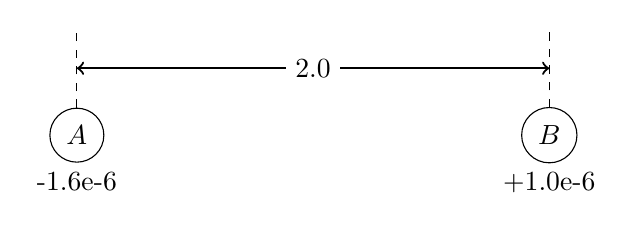
\begin{tikzpicture}
    %% nodes
    \node[draw,circle,anchor=center] (A) at (-3,0) {$A$};
    \node[draw,circle,anchor=center] (B) at (+3,0) {$B$};
    %% labels
    \node[anchor=north] at (A.south) {\SI{-1.6e-6}{\coulomb}};
    \node[anchor=north] at (B.south) {\SI{+1.0e-6}{\coulomb}};
    %% distance
    \draw[dashed] (A.north) -- ++(90:1);
    \draw[dashed] (B.north) -- ++(90:1);
    \draw[thick,<->] (A.north) ++ (90:0.5) -- ++(0:6)
        node[pos=0.5,anchor=center,fill=white] {\SI{2.0}{\meter}};
\end{tikzpicture}
}

\element{nysed}{
\begin{question}{June2015-Q30}
    %Base your answers to questions 30 and 31 on the diagram below and on your knowledge of physics. 
    The diagram represents two small, charged,
        identical metal spheres, $A$ and $B$ that are separated by a distance of \SI{2.0}{\meter}.
    \begin{center}
        \JuneTwentyFifteenQThirty
    \end{center}
    What is the magnitude of the electrostatic force exerted by sphere $A$ on sphere $B$?
    \begin{multicols}{2}
    \begin{choices}
        \wrongchoice{\SI{7.2e-3}{\newton}}
        \wrongchoice{\SI{3.6e-3}{\newton}}
        \wrongchoice{\SI{8.0e-13}{\newton}}
        \wrongchoice{\SI{4.0e-13}{\newton}}
    \end{choices}
    \end{multicols}
\end{question}
}

\element{nysed}{
\begin{question}{June2015-Q31}
    The diagram represents two small, charged,
        identical metal spheres, $A$ and $B$ that are separated by a distance of \SI{2.0}{\meter}.
    \begin{center}
        \JuneTwentyFifteenQThirty
    \end{center}
    If the two spheres were touched together and then separated,
        the charge on sphere $A$ would be:
    \begin{multicols}{2}
    \begin{choices}
        \wrongchoice{\SI{-3.0e-7}{\coulomb}}
        \wrongchoice{\SI{-6.0e-6}{\coulomb}}
        \wrongchoice{\SI{-1.3e-6}{\coulomb}}
        \wrongchoice{\SI{-2.6e-6}{\coulomb}}
    \end{choices}
    \end{multicols}
\end{question}
}


%% Section June2014
%%--------------------
\element{nysed}{
\begin{question}{June2014-Q12}
    A beam of electrons passes through an electric field where the magnitude of the electric field strength is \SI{3.00e3}{\newton\per\coulomb}.
    What is the magnitude of the electrostatic force exerted by the electric field on each electron in the beam?
    \begin{multicols}{2}
    \begin{choices}
      \correctchoice{\SI{4.8e-16}{\newton}}
        \wrongchoice{\SI{5.33e-23}{\newton}}
        \wrongchoice{\SI{3.00e3}{\newton}}
        \wrongchoice{\SI{1.88e22}{\newton}}
    \end{choices}
    \end{multicols}
\end{question}
}

\element{nysed}{
\begin{question}{June2014-Q13}
    How much work is required to move \SI{3.0}{\coulomb} of electric charge a distance of \SI{0.010}{\meter} through a potential difference of \SI{9.0}{\volt}
    \begin{multicols}{2}
    \begin{choices}
      \correctchoice{\SI{27}{\joule}}
        \wrongchoice{\SI{2.7e3}{\joule}}
        \wrongchoice{\SI{3.0}{\joule}}
        \wrongchoice{\SI{3.0e-2}{\joule}}
    \end{choices}
    \end{multicols}
\end{question}
}

\element{nysed}{
\begin{question}{June2014-Q32}
    Two identically-sized metal spheres, $A$ and $B$, are on insulating stands,
        as shown in the diagram below.
    Sphere $A$ possesses an excess of \num{6.3e10} electrons and sphere $B$ is neutral.
    \begin{center}
    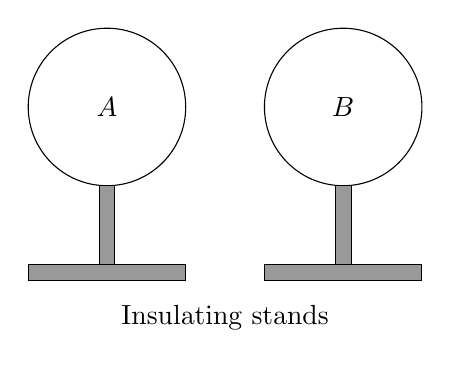
\begin{tikzpicture}
        \begin{scope}[xshift=-1.5cm]
            \draw (0,0) circle (1cm);
            \node[anchor=center] at (0,0) {$A$};
            \draw[fill=white!60!black] (-0.1,-1) rectangle (0.1,-2);
            \draw[fill=white!60!black] (-1,-2) rectangle (1,-2.2);
        \end{scope}
        \begin{scope}[xshift=+1.5cm]
            \draw (0,0) circle (1cm);
            \node[anchor=center] at (0,0) {$B$};
            \draw[fill=white!60!black] (-0.1,-1) rectangle (0.1,-2);
            \draw[fill=white!60!black] (-1,-2) rectangle (1,-2.2);
        \end{scope}
        \node[anchor=north] at (0,-2.4) {Insulating stands};
    \end{tikzpicture}
    \end{center}
    Which diagram best represents the charge distribution on sphere $B$?
    \begin{multicols}{2}
    \begin{choices}[o]
        \AMCboxDimensions{down=-1.5cm}
        \wrongchoice{
            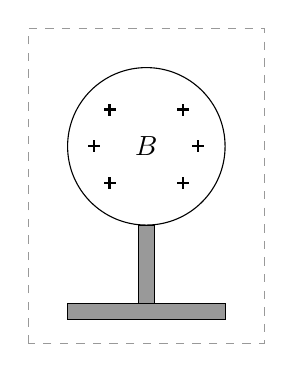
\begin{tikzpicture}
                \draw[dashed,white!60!black] (-1.5,-2.5) rectangle (1.5,1.5);
                \draw (0,0) circle (1cm);
                \node[anchor=center] at (0,0) {$B$};
                \draw[fill=white!60!black] (-0.1,-1) rectangle (0.1,-2);
                \draw[fill=white!60!black] (-1,-2) rectangle (1,-2.2);
                %% left and right positive
                \foreach \x in {-45,0,45,135,180,225}
                    \foreach \y in {0,90,180,270} {
                        \draw[thick] (\x:0.66) -- ++(\y:0.5ex);
                        \draw[thick] (\x:0.66) -- ++(\y:0.5ex);
                    }
            \end{tikzpicture}
        }
        \wrongchoice{
            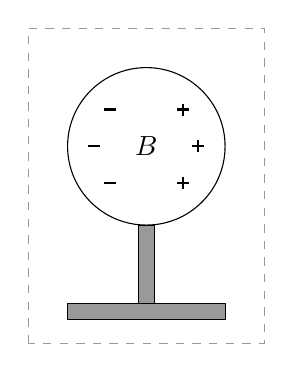
\begin{tikzpicture}
                \draw[dashed,white!60!black] (-1.5,-2.5) rectangle (1.5,1.5);
                \draw (0,0) circle (1cm);
                \node[anchor=center] at (0,0) {$B$};
                \draw[fill=white!60!black] (-0.1,-1) rectangle (0.1,-2);
                \draw[fill=white!60!black] (-1,-2) rectangle (1,-2.2);
                %% left negative
                \foreach \x in {135,180,225}
                    \foreach \y in {0,180} {
                        \draw[thick] (\x:0.66) -- ++(\y:0.5ex);
                        \draw[thick] (\x:0.66) -- ++(\y:0.5ex);
                    }
                %% right positive
                \foreach \x in {-45,0,45}
                    \foreach \y in {0,90,180,270} {
                        \draw[thick] (\x:0.66) -- ++(\y:0.5ex);
                        \draw[thick] (\x:0.66) -- ++(\y:0.5ex);
                    }
            \end{tikzpicture}
        }
        \wrongchoice{
            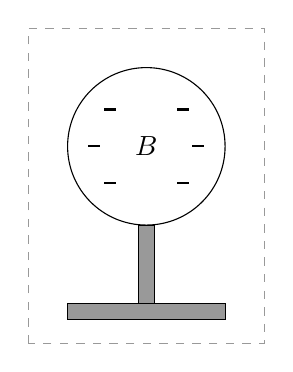
\begin{tikzpicture}
                \draw[dashed,white!60!black] (-1.5,-2.5) rectangle (1.5,1.5);
                \draw (0,0) circle (1cm);
                \node[anchor=center] at (0,0) {$B$};
                \draw[fill=white!60!black] (-0.1,-1) rectangle (0.1,-2);
                \draw[fill=white!60!black] (-1,-2) rectangle (1,-2.2);
                %% left and right negative
                \foreach \x in {-45,0,45,135,180,225}
                    \foreach \y in {0,180} {
                        \draw[thick] (\x:0.66) -- ++(\y:0.5ex);
                        \draw[thick] (\x:0.66) -- ++(\y:0.5ex);
                    }
            \end{tikzpicture}
        }
        \correctchoice{
            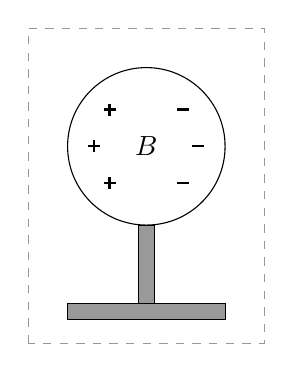
\begin{tikzpicture}
                \draw[dashed,white!60!black] (-1.5,-2.5) rectangle (1.5,1.5);
                \draw (0,0) circle (1cm);
                \node[anchor=center] at (0,0) {$B$};
                \draw[fill=white!60!black] (-0.1,-1) rectangle (0.1,-2);
                \draw[fill=white!60!black] (-1,-2) rectangle (1,-2.2);
                %% left positive
                \foreach \x in {135,180,225}
                    \foreach \y in {0,90,180,270} {
                        \draw[thick] (\x:0.66) -- ++(\y:0.5ex);
                        \draw[thick] (\x:0.66) -- ++(\y:0.5ex);
                    }
                %% right negative
                \foreach \x in {-45,0,45}
                    \foreach \y in {0,180} {
                        \draw[thick] (\x:0.66) -- ++(\y:0.5ex);
                        \draw[thick] (\x:0.66) -- ++(\y:0.5ex);
                    }
            \end{tikzpicture}
        }
    \end{choices}
    \end{multicols}
\end{question}
}

\element{nysed}{
\begin{question}{June2014-Q33}
    Two points, $A$ and $B$, are located within the electric field produced by a \SI{-3.0}{\nano\coulomb} charge.
    Point $A$ is \SI{0.10}{\meter} to the left of the charge and point $B$ is \SI{0.20}{\meter} to the right of the charge,
        as shown in the diagram below.
    \begin{center}
    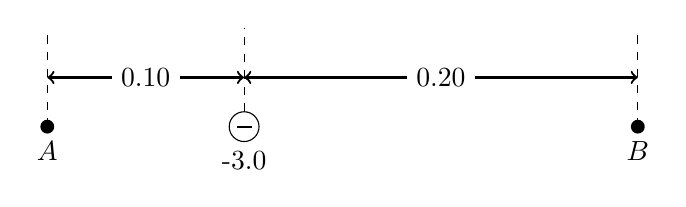
\begin{tikzpicture}[scale=1.25]
        %% points
        \fill (-2,0) circle (2pt) node[anchor=north,yshift=-2pt] {$A$};
        \fill (+4,0) circle (2pt) node[anchor=north,yshift=-2pt] {$B$};
        %% distances
        \draw[dashed] (-2,0) -- (-2,1);
        \draw[dashed] (+4,0) -- (+4,1);
        \draw[dashed] (0,1ex) -- (0,1);
        \draw[thick,<->] (-2,0.5) -- (0,0.5) node[pos=0.5,anchor=center,fill=white] {\SI{0.10}{\meter}};
        \draw[thick,<->] (+4,0.5) -- (0,0.5) node[pos=0.5,anchor=center,fill=white] {\SI{0.20}{\meter}};
        %% charge
        \draw (0,0) circle (1ex);
        \draw[thick] (0,0) -- (0:0.5ex);
        \draw[thick] (0,0) -- (180:0.5ex);
        \node[anchor=north] at (0,-1ex) {\SI{-3.0}{\nano\coulomb}};
    \end{tikzpicture}
    \end{center}
    Compared to the magnitude of the electric field strength at points $A$,
        the magnitude of the electric field strength at point $B$ is:
    \begin{choices}
      \correctchoice{one-fourth as great}
        \wrongchoice{four times as great}
        \wrongchoice{half as great}
        \wrongchoice{twice as great}
    \end{choices}
\end{question}
}

\element{nysed}{
\begin{question}{June2014-Q37}
    Two identically-sized metal spheres on insulating stands are positioned as shown below.
    The charge on sphere $A$ is \SI{-4.0e-6}{\coulomb} and the charge on sphere $B$ is \SI{-8.0e-6}{\coulomb}.
    \begin{center}
    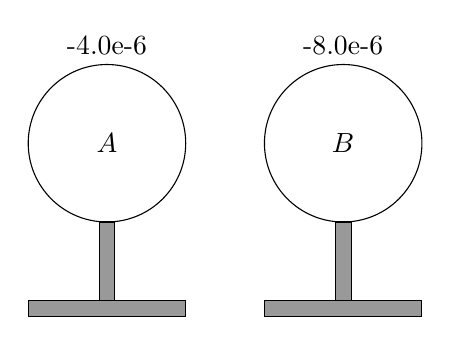
\begin{tikzpicture}
        \begin{scope}[xshift=-1.5cm]
            \draw (0,0) circle (1cm);
            \node[anchor=center] at (0,0) {$A$};
            \draw[fill=white!60!black] (-0.1,-1) rectangle (0.1,-2);
            \draw[fill=white!60!black] (-1,-2) rectangle (1,-2.2);
            \node[anchor=south] at (0,1) {\SI{-4.0e-6}{\coulomb}};
        \end{scope}
        \begin{scope}[xshift=+1.5cm]
            \draw (0,0) circle (1cm);
            \node[anchor=center] at (0,0) {$B$};
            \draw[fill=white!60!black] (-0.1,-1) rectangle (0.1,-2);
            \draw[fill=white!60!black] (-1,-2) rectangle (1,-2.2);
            \node[anchor=south] at (0,1) {\SI{-8.0e-6}{\coulomb}};
        \end{scope}
    \end{tikzpicture}
    \end{center}
    The two spheres are touched together and then separated.
    The total number of excess electrons on sphere $A$ after the separation is:
    \begin{multicols}{2}
    \begin{choices}
      \correctchoice{\num{3.8e13}}
        \wrongchoice{\num{2.5e13}}
        \wrongchoice{\num{5.0e13}}
        \wrongchoice{\num{7.5e13}}
    \end{choices}
    \end{multicols}
\end{question}
}

\element{nysed}{
\begin{question}{June2014-Q39}
    Which combination of units can be used to express electrical energy?
    \begin{choices}
        \wrongchoice{volt per coulomb (\si{\volt\per\coulomb})}
        \wrongchoice{coulomb per volt (\si{\coulomb\per\volt})}
      \correctchoice{volt coulomb (\si{\volt\coulomb})}
        \wrongchoice{volt coulomb second (\si{\volt\coulomb\second})}
    \end{choices}
\end{question}
}


%% Section June2013
%%--------------------
\element{nysed}{
\begin{question}{June2013-Q23}
    A dry plastic rod is rubbed with cool cloth and then held near a thin stream of water from a faucet.
    The path of the stream of water is changed,
        as represented in the diagram below.
    \begin{center}
        \includegraphics[keepaspectratio,scale=0.75]{June2013-Q23}
    \end{center}
    Which force causes the path of the stream of water to change due to the plastic rod?
    \begin{multicols}{2}
    \begin{choices}
        \wrongchoice{nuclear}
        \wrongchoice{magnetic}
      \correctchoice{electrostatic}
        \wrongchoice{gravitational}
    \end{choices}
    \end{multicols}
\end{question}
}

\element{nysed}{
\begin{question}{June2013-Q27}
    The electronvolt (\si{\eV}) is a unit of:
    \begin{choices}
      \correctchoice{energy}
        \wrongchoice{charge}
        \wrongchoice{electric field strength}
        \wrongchoice{electric potential difference}
    \end{choices}
\end{question}
}

\element{nysed}{
\begin{question}{June2013-Q33}
    Which net charge could be found on an object?
    \begin{multicols}{2}
    \begin{choices}
      \correctchoice{\SI[retain-explicit-plus]{+4.80e-19}{\coulomb}}
        \wrongchoice{\SI[retain-explicit-plus]{+2.40e-19}{\coulomb}}
        \wrongchoice{\SI{-2.40e-19}{\coulomb}}
        \wrongchoice{\SI{-5.60e-19}{\coulomb}}
    \end{choices}
    \end{multicols}
\end{question}
}

\element{nysed}{
\begin{question}{June2013-Q41}
    An electron is located in an electric field of magnitude \SI{600}{\newton\per\coulomb}.
    What is the magnitude of the electrostatic force acting on the electron?
    \begin{multicols}{2}
    \begin{choices}
        \wrongchoice{\SI{3.75e21}{\newton}}
        \wrongchoice{\SI{6.00e2}{\newton}}
      \correctchoice{\SI{9.6e-17}{\newton}}
        \wrongchoice{\SI{2.67e-22}{\newton}}
    \end{choices}
    \end{multicols}
\end{question}
}

\element{nysed}{
\begin{question}{June2013-Q43}
    When two point charges of magnitude of $q_1$ and $q_2$ are separated by a distance, $r$, the magnitude of the electrostatic force between them is $F$.
    What would be the magnitude of the electrostatic force between point charges $2q_1$ and $4q_2$ when separated by a distance of $2r$?
    \begin{multicols}{4}
    \begin{choices}
        \wrongchoice{$F$}
      \correctchoice{$2F$}
        \wrongchoice{$16F$}
        \wrongchoice{$4F$}
    \end{choices}
    \end{multicols}
\end{question}
}

\element{nysed}{
\begin{question}{June2013-Q46}
    Which diagram best represents the electric field between two oppositely charged conducting spheres?
    \begin{multicols}{2}
    \begin{choices}
        \AMCboxDimensions{down=-1.5em}
        \wrongchoice{\includegraphics[keepaspectratio,scale=0.75]{June2013-Q46-A}}
        \wrongchoice{\includegraphics[keepaspectratio,scale=0.75]{June2013-Q46-B}}
      \correctchoice{\includegraphics[keepaspectratio,scale=0.75]{June2013-Q46-C}}
        \wrongchoice{\includegraphics[keepaspectratio,scale=0.75]{June2013-Q46-D}}
    \end{choices}
    \end{multicols}
\end{question}
}


%% Section June2012
%%--------------------
\element{nysed}{
\begin{question}{June2012-Q04}
    A particle could have a charge of:
    \begin{multicols}{2}
    \begin{choices}
        \wrongchoice{\SI{0.80e-19}{\coulomb}}
        \wrongchoice{\SI{1.2e-19}{\coulomb}}
      \correctchoice{\SI{3.2e-19}{\coulomb}}
        \wrongchoice{\SI{4.1e-19}{\coulomb}}
    \end{choices}
    \end{multicols}
\end{question}
}

\element{nysed}{
\begin{question}{June2012-Q18}
    Two electrons are separated by a distance of \SI{3.00e-6}{\meter}.
    What are the magnitudes and direction of the electrostatic forces each exerts on the other?
    \begin{choices}
      \correctchoice{\SI{2.56e-17}{\newton} away from each other}
        \wrongchoice{\SI{2.56e-17}{\newton} toward each other}
        \wrongchoice{\SI{7.67e-23}{\newton} away from each other}
        \wrongchoice{\SI{7.67e-23}{\newton} toward each other}
    \end{choices}
\end{question}
}

\element{nysed}{
\begin{question}{June2012-Q19}
    Which object will have the greatest change in electrical energy?
    \begin{choices}
        \wrongchoice{an electron moved through a potential difference of \SI{2.0}{\volt}}
        \wrongchoice{a metal sphere with charge of \SI{1.0e-9}{\coulomb} moved through a potential difference of \SI{2.0}{\volt}}
        \wrongchoice{an electron moved through a potential difference of \SI{4.0}{\volt}}
      \correctchoice{a metal sphere with charge of \SI{1.0e-9}{\coulomb} moved through a potential difference of \SI{4.0}{\volt}}
    \end{choices}
\end{question}
}

\element{nysed}{
\begin{question}{June2012-Q28}
    A \SI{3.00e-9}{\coulomb} test charge is placed near a negatively charged metal sphere.
    The sphere exerts an electrostatic force of magnitude \SI{6.00e-5}{\newton} on the test charge.
    What is the magnitude and direction of the electric field strength at this location?
    \begin{choices}
        \wrongchoice{\SI{2.00e4}{\newton\per\coulomb} directed away from the sphere}
      \correctchoice{\SI{2.00e4}{\newton\per\coulomb} directed toward the sphere}
        \wrongchoice{\SI{5.00e-5}{\newton\per\coulomb} directed away from the sphere}
        \wrongchoice{\SI{5.00e-5}{\newton\per\coulomb} directed toward the sphere}
    \end{choices}
\end{question}
}


%% Section June2011
%%--------------------
\element{nysed}{
\begin{question}{June2011-Q15}
    Which diagram represents the electric field lines between two small
        electrically charged spheres?
    \begin{multicols}{2}
    \begin{choices}
        \AMCboxDimensions{down=-1.5em}
        \wrongchoice{\includegraphics[keepaspectratio,scale=0.60]{June2011-Q15-A}}
      \correctchoice{\includegraphics[keepaspectratio,scale=0.60]{June2011-Q15-B}}
        \wrongchoice{\includegraphics[keepaspectratio,scale=0.60]{June2011-Q15-C}}
        \wrongchoice{\includegraphics[keepaspectratio,scale=0.60]{June2011-Q15-D}}
    \end{choices}
    \end{multicols}
\end{question}
}

\element{nysed}{
\begin{question}{June2011-Q17}
    Two metal spheres, $A$ and $B$, posses charges of \SI{1.0}{\micro\coulomb} and \SI{2.0}{\micro\coulomb}, respectively.
    In the diagram below, arrow $F$ represents the electrostatic force exerted on sphere $B$ by sphere $A$.
    \begin{center}
    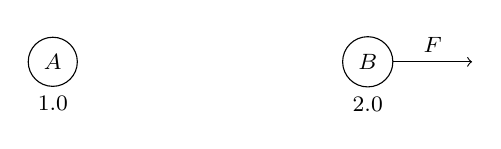
\begin{tikzpicture}[font=\footnotesize]
        \node[draw,circle,minimum size=0.50cm,anchor=center] (A) at (-2,0) {$A$};
        \node[draw,circle,minimum size=0.50cm,anchor=center] (B) at (+2,0) {$B$};
        \node[anchor=north] at (A.south) {\SI{1.0}{\micro\coulomb}};
        \node[anchor=north] at (B.south) {\SI{2.0}{\micro\coulomb}};
        \draw[->] (B.east) -- ++(0:1cm) node[pos=0.5,anchor=south] {$F$};
    \end{tikzpicture}
    \end{center}
    Which arrow represents the magnitude and direction of the electrostatic force exerted on sphere $A$ by sphere $B$?
    \begin{multicols}{2}
    \begin{choices}\small
        \AMCboxDimensions{down=-0.25cm}
        \correctchoice{
            \begin{tikzpicture}
                \draw[dashed,white!60!black] (-0.5,-0.5) rectangle (2.50,0.5);
                \draw[<-] (0,0) -- (1.00,0) node[pos=0.5,anchor=south] {$F$};
            \end{tikzpicture}
        }
        \wrongchoice{
            \begin{tikzpicture}
                \draw[dashed,white!60!black] (-0.5,-0.5) rectangle (2.50,0.5);
                \draw[->] (0,0) -- (1.00,0) node[pos=0.5,anchor=south] {$F$};
            \end{tikzpicture}
        }
        \wrongchoice{
            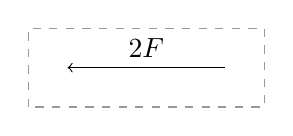
\begin{tikzpicture}
                \draw[dashed,white!60!black] (-0.5,-0.5) rectangle (2.50,0.5);
                \draw[<-] (0,0) -- (2.00,0) node[pos=0.5,anchor=south] {$2F$};
            \end{tikzpicture}
        }
        \wrongchoice{
            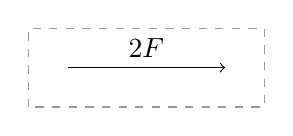
\begin{tikzpicture}
                \draw[dashed,white!60!black] (-0.5,-0.5) rectangle (2.50,0.5);
                \draw[->] (0,0) -- (2.00,0) node[pos=0.5,anchor=south] {$2F$};
            \end{tikzpicture}
        }
    \end{choices}
    \end{multicols}
\end{question}
}

\element{nysed}{
\begin{question}{June2011-Q18}
    The diagram below represents a positively charged particle about to enter the electric field between two oppositely charged parallel plates.
    \begin{center}
    \begin{tikzpicture}
        %% charged particle
        \foreach \y in {0,90,180,270} \draw[thick] (7,1.5) -- ++ (\y:0.1);
        \draw (7,1.5) circle (0.2);
        \draw[thick,->] (6.8,1.5) -- (5.5,1.5) node[pos=0.5,anchor=south] {$v$};
        %% Bottom negative
        \draw (0,0) rectangle (6,-1em);
        \foreach \x in {2,6,...,58}
            \foreach \y in {0,180} {
                \draw (\x mm,-0.5em) -- ++(\y:0.5ex);
            }
        %% Top positive
        \draw (0,3) rectangle (6,3cm+1em);
        \foreach \x in {2,6,...,58}
            \foreach \y in {0,90,180,270} {
                \draw (\x mm,3cm+0.5em) -- ++(\y:0.5ex);
            }
    \end{tikzpicture}
    \end{center}
    The electric field will deflect the particle:
    \begin{choices}
        \wrongchoice{into the page}
        \wrongchoice{out of the page}
        \wrongchoice{toward the top of the page}
      \correctchoice{toward the bottom of the page}
    \end{choices}
\end{question}
}

\element{nysed}{
\begin{question}{June2011-Q19}
    What is the total amount of work required to move a proton through a potential difference of \SI{100}{\volt}?
    \begin{multicols}{2}
    \begin{choices}
        \wrongchoice{\SI{1.60e-21}{\joule}}
      \correctchoice{\SI{1.60e-17}{\joule}}
        \wrongchoice{\SI{1.00e2}{\joule}}
        \wrongchoice{\SI{6.25e20}{\joule}}
    \end{choices}
    \end{multicols}
\end{question}
}

\element{nysed}{
\begin{question}{June2011-Q40}
    The diagram below shows the arrangement of three small spheres,
        $A$, $B$, and $C$, having charges of $3q$, $q$, and $q$, respectively.
    Spheres $A$ and $C$ are located distance $r$ from sphere $B$.
    \begin{center}
        %% NOTE: tikz, easy
        %\includegraphics[keepaspectratio,scale=0.75]{June2011-Q40}
    \end{center}
    Compared to the magnitude of the electrostatic force exerted by sphere $B$ on sphere $C$,
        the magnitude of the electrostatic force by sphere $A$ on sphere $C$ is:
    \begin{multicols}{2}
    \begin{choices}
        \wrongchoice{the same}
        \wrongchoice{twice as great}
      \correctchoice{\num{3/4} as great}
        \wrongchoice{\num{3/2} as great}
    \end{choices}
    \end{multicols}
\end{question}
}

\element{nysed}{
\begin{question}{June2011-Q43}
    Two parallel metal plates are connected to a variable source of potential difference.
    When the potential difference of the source is increased,
        the magnitude of the field strength between the plates increases.
    The diagram below shows an electron located between the plates.
    \begin{center}
        \includegraphics[keepaspectratio,scale=0.70]{June2011-Q43}
    \end{center}
    Which graph represents the relationship between the magnitude of the electrostatic force on the electron and the magnitude of the electric field strength between the plate?
    \begin{multicols}{2}
    \begin{choices}
        \AMCboxDimensions{down=-2.5em}
        \correctchoice{
            \begin{tikzpicture}
                \begin{axis}[
                    axis y line=left,
                    axis x line=bottom,
                    axis line style={->},
                    xlabel={electric field},
                    xtick=\empty,
                    ylabel={force},
                    ytick=\empty,
                    xmin=0,xmax=11,
                    ymin=0,ymax=11,
                    width=\columnwidth,
                    very thin,
                ]
                \addplot[line width=1pt,domain=0:10]{x};
                \end{axis}
            \end{tikzpicture}
        }
        \wrongchoice{
            \begin{tikzpicture}
                \begin{axis}[
                    axis y line=left,
                    axis x line=bottom,
                    axis line style={->},
                    xlabel={electric field},
                    xtick=\empty,
                    ylabel={force},
                    ytick=\empty,
                    xmin=0,xmax=11,
                    ymin=0,ymax=11,
                    width=\columnwidth,
                    very thin,
                ]
                \addplot[line width=1pt,domain=0:10]{10/x^2};
                \end{axis}
            \end{tikzpicture}
        }
        \wrongchoice{
            \begin{tikzpicture}
                \begin{axis}[
                    axis y line=left,
                    axis x line=bottom,
                    axis line style={->},
                    xlabel={electric field},
                    xtick=\empty,
                    ylabel={force},
                    ytick=\empty,
                    xmin=0,xmax=11,
                    ymin=0,ymax=11,
                    width=\columnwidth,
                    very thin,
                ]
                \addplot[line width=1pt,domain=0:10]{8};
                \end{axis}
            \end{tikzpicture}
        }
        \wrongchoice{
            \begin{tikzpicture}
                \begin{axis}[
                    axis y line=left,
                    axis x line=bottom,
                    axis line style={->},
                    xlabel={electric field},
                    xtick=\empty,
                    ylabel={force},
                    ytick=\empty,
                    xmin=0,xmax=11,
                    ymin=0,ymax=11,
                    width=\columnwidth,
                    very thin,
                ]
                \addplot[line width=1pt,domain=0:10]{0.1*x*x};
                \end{axis}
            \end{tikzpicture}
        }
    \end{choices}
    \end{multicols}
\end{question}
}


%% Section June2010
%%--------------------
\element{nysed}{
\begin{question}{June2010-Q21}
    What is the magnitude of the electrostatic force between two electrons separated by a distance of \SI{1.00e-8}{\meter}?
    \begin{multicols}{2}
    \begin{choices}
        \wrongchoice{\SI{2.56e-22}{\newton}}
        \wrongchoice{\SI{2.30e-20}{\newton}}
      \correctchoice{\SI{2.30e-12}{\newton}}
        \wrongchoice{\SI{1.44e-1}{\newton}}
    \end{choices}
    \end{multicols}
\end{question}
}

\element{nysed}{
\begin{question}{June2010-Q22}
    The diagram below represents the electric field surrounding two charged spheres, $A$ and $B$.
    \begin{center}
        \includegraphics[keepaspectratio,scale=0.75]{June2010-Q22}
    \end{center}
    What is the sign of the charge of each sphere?
    \begin{choices}
        \wrongchoice{Sphere $A$ is positive and sphere $B$ is negative.}
      \correctchoice{Sphere $A$ is negative and sphere $B$ is positive.}
        \wrongchoice{Both spheres are positive.}
        \wrongchoice{Both spheres are negative.}
    \end{choices}
\end{question}
}

\element{nysed}{
\begin{question}{June2010-Q37}
    Which electrical unit is equivalent to one joule?
    \begin{choices}
        \wrongchoice{volt per meter (\si{\volt\per\meter})}
        \wrongchoice{ampere volt (\si{\ampere\volt})}
        \wrongchoice{volt per coulomb (\si{\volt\per\coulomb})}
      \correctchoice{coulomb volt (\si{\coulomb\volt})}
    \end{choices}
\end{question}
}


\element{nysed}{
\begin{question}{June2010-Q47}
    The distance between an electron and a proton is varied.
    Which pair of graphs best represents the relationship between gravitational force, $F_g$,
        and distance, $r$, and the relationship between electrostatic force, $F_e$, and distance, $r$, for these particles?
    %% NOTE: consider ylabel={electrostatic} or {gravitaitonal}
    \begin{choices}
        \AMCboxDimensions{down=-2.5em}
        \correctchoice{
            \begin{tikzpicture}
                \begin{groupplot}[
                        axis y line=left,
                        axis x line=bottom,
                        axis line style={->},
                        y label style={rotate=270},
                        group style={group size=2 by 1},
                        xtick=\empty,
                        ytick=\empty,
                        xmin=0,xmax=11,
                        ymin=0,ymax=11,
                        width=0.5\columnwidth,
                    ]
                    \nextgroupplot[
                        xlabel={$r$},
                        ylabel={$F_g$},
                    ] \addplot[line width=1pt,domain=0:10] {10/x};
                    \nextgroupplot[
                        xlabel={$r$},
                        ylabel={$F_e$},
                    ] \addplot[line width=1pt,domain=0:10] {10/x};
                \end{groupplot}
            \end{tikzpicture}
        }
        \wrongchoice{
            \begin{tikzpicture}
                \begin{groupplot}[
                        axis y line=left,
                        axis x line=bottom,
                        axis line style={->},
                        y label style={rotate=270},
                        group style={group size=2 by 1},
                        xtick=\empty,
                        ytick=\empty,
                        xmin=0,xmax=11,
                        ymin=0,ymax=11,
                        width=0.5\columnwidth,
                    ]
                    \nextgroupplot[
                        xlabel={$r$},
                        ylabel={$F_g$},
                    ] \addplot[line width=1pt,domain=0:10] {10/x};
                    \nextgroupplot[
                        xlabel={$r$},
                        ylabel={$F_e$},
                    ] \addplot[line width=1pt,domain=0:10] {0.1*x*x};
                \end{groupplot}
            \end{tikzpicture}
        }
        \wrongchoice{
            \begin{tikzpicture}
                \begin{groupplot}[
                        axis y line=left,
                        axis x line=bottom,
                        axis line style={->},
                        y label style={rotate=270},
                        group style={group size=2 by 1},
                        xtick=\empty,
                        ytick=\empty,
                        xmin=0,xmax=11,
                        ymin=0,ymax=11,
                        width=0.5\columnwidth,
                    ]
                    \nextgroupplot[
                        xlabel={$r$},
                        ylabel={$F_g$},
                    ] \addplot[line width=1pt,domain=0:10] {0.1*x*x};
                    \nextgroupplot[
                        xlabel={$r$},
                        ylabel={$F_e$},
                    ] \addplot[line width=1pt,domain=0:10] {0.1*x*x};
                \end{groupplot}
            \end{tikzpicture}
        }
        \wrongchoice{
            \begin{tikzpicture}
                \begin{groupplot}[
                        axis y line=left,
                        axis x line=bottom,
                        axis line style={->},
                        y label style={rotate=270},
                        group style={group size=2 by 1},
                        xtick=\empty,
                        ytick=\empty,
                        xmin=0,xmax=11,
                        ymin=0,ymax=11,
                        width=0.5\columnwidth,
                    ]
                    \nextgroupplot[
                        xlabel={$r$},
                        ylabel={$F_g$},
                    ] \addplot[line width=1pt,domain=0:10] {0.1*x*x};
                    \nextgroupplot[
                        xlabel={$r$},
                        ylabel={$F_e$},
                    ] \addplot[line width=1pt,domain=0:10] {10/x};
                \end{groupplot}
            \end{tikzpicture}
        }
    \end{choices}
\end{question}
}


%% Section June2009
%%--------------------
\element{nysed}{
\begin{question}{June2009-Q17}
    A distance of \SI{1.0}{\meter} separates the centers of two small charged spheres.
    The spheres exert gravitational force $F_g$ and electrostatic force $F_e$ on each other.
    If the distance between the spheres centers is increases to \SI{3.0}{\meter},
        the gravitational force and the electrostatic force, respectively, may be represented as:
    \begin{multicols}{2}
    \begin{choices}
      \correctchoice{$\dfrac{F_g}{9}$ and $\dfrac{F_e}{9}$}
        \wrongchoice{$\dfrac{F_g}{3}$ and $\dfrac{F_e}{3}$}
        \wrongchoice{$3 F_g$ and $3 F_e$}
        \wrongchoice{$9 F_g$ and $9 F_e$}
    \end{choices}
    \end{multicols}
\end{question}
}

\element{nysed}{
\begin{question}{June2009-Q21}
    A beam of electrons is directed into the electric field between two oppositely charged parallel plates,
        as shown in the diagram below.
    \begin{center}
    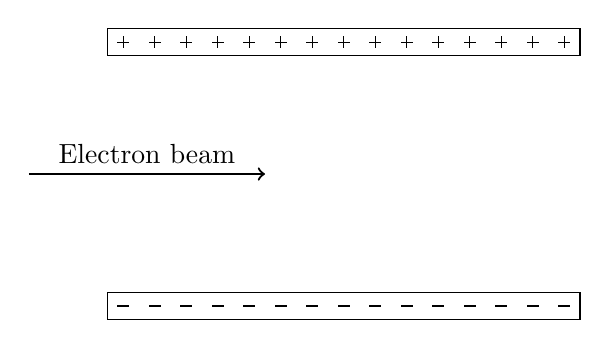
\begin{tikzpicture}
        %% Electron Vector
        \draw[thick,->] (-1,1.5) -- ++(0:3) node[pos=0.5,anchor=south] {Electron beam};
        %% Bottom
        \draw (0,0) rectangle (6,-1em);
        \foreach \x in {2,6,...,58}
            \foreach \y in {0,90,180,270} {
                \draw (\x mm,3cm+0.5em) -- ++(\y:0.5ex);
            }
        %% Top
        \draw (0,3) rectangle (6,3cm+1em);
        \foreach \x in {2,6,...,58}
            \foreach \y in {0,180} {
                \draw (\x mm,-0.5em) -- ++(\y:0.5ex);
            }
    \end{tikzpicture}
    \end{center}
    The electrostatic force exerted on the electrons by the electric field is directed:
    \begin{choices}
        \wrongchoice{into the page}
        \wrongchoice{out of the page}
        \wrongchoice{toward the bottom of the page}
      \correctchoice{toward the top of the page}
    \end{choices}
\end{question}
}


%% Section Jan2009
%%--------------------
\element{nysed}{
\begin{question}{Jan2009-Q19}
    The diagram below shows a beam of electrons fired through the region between two oppositely charged parallel plates in a cathode ray tube.
    \begin{center}
        \includegraphics[keepaspectratio,width=0.95\linewidth]{Jan2009-Q19}
    \end{center}
    After passing between the charged plates,
        the electrons will most likely travel path:
    \begin{multicols}{4}
    \begin{choices}[o]
      \correctchoice{$A$}
        \wrongchoice{$B$}
        \wrongchoice{$C$}
        \wrongchoice{$D$}
    \end{choices}
    \end{multicols}
\end{question}
}

\element{nysed}{
\begin{question}{Jan2009-Q34}
    If an object has a net negative charge of \SI{4.0}{\coulomb},
        the object possesses:
    \begin{choices}
        \wrongchoice{\num{6.3e19} more electrons than protons}
      \correctchoice{\num{2.5e19} more electrons than protons}
        \wrongchoice{\num{6.3e18} more protons than electrons}
        \wrongchoice{\num{2.5e18} more protons than electrons}
    \end{choices}
\end{question}
}


%% Section June2008
%%--------------------
\element{nysed}{
\begin{question}{June2008-Q22}
    An electron is located in the electric field between two parallel metal plates as shown in the diagram below.
    \begin{center}
    \ctikzset{bipoles/length=0.75cm}
    \begin{circuitikz}
        \draw (1,-1) to [battery,l=\SI{40.0}{\volt}] (1,1);
    \end{circuitikz}
    \includegraphics[keepaspectratio,scale=0.75]{June2008-Q22}
    \end{center}
    If the electron is attracted to plate $A$, then plate $A$ is charged:
    \begin{choices}
      \correctchoice{positively, and the electric field is directed from plate $A$ toward plate $B$}
        \wrongchoice{positively, and the electric field is directed from plate $B$ toward plate $A$}
        \wrongchoice{negatively, and the electric field is directed from plate $A$ toward plate $B$}
        \wrongchoice{negatively, and the electric field is directed from plate $B$ toward plate $A$}
    \end{choices}
\end{question}
}


%% Section Jan2008
%%--------------------
\element{nysed}{
\begin{question}{Jan2008-Q19}
    The diagram below represents an electron within an electric field between two parallel plates that are charged with a potential difference of \SI{40.0}{\volt}.
    \begin{center}
    \ctikzset{bipoles/length=0.75cm}
    \begin{circuitikz}
        %% voltage
        \draw (1,1) to [battery,l=\SI{40.0}{\volt}] (1,-1);
        %% plates
        \draw (-4,1.05) rectangle (0,0.95);
        \draw (0,1) -- (1,1);
        \draw (-4,-1.05) rectangle (0,-0.95);
        \draw (0,-1) -- (1,-1);
        %% charge
        \draw[thick,xshift=-2cm] (-0.5ex,0) -- (0.5ex,0);
        \draw[xshift=-2cm] (0,0) circle (1ex);
    \end{circuitikz}
    \end{center}
    If the magnitude of the electric force on the electron is \SI{2.00e-15}{\newton},
        the magnitude of the electric field strength between the charged plates is:
    \begin{multicols}{2}
    \begin{choices}
        \wrongchoice{\SI{3.20e-34}{\newton\per\coulomb}}
        \wrongchoice{\SI{2.00e-14}{\newton\per\coulomb}}
      \correctchoice{\SI{1.24e4}{\newton\per\coulomb}}
        \wrongchoice{\SI{2.00e16}{\newton\per\coulomb}}
    \end{choices}
    \end{multicols}
\end{question}
}

\element{nysed}{
\begin{question}{Jan2008-Q30}
    A subatomic particle could have a charge of:
    \begin{multicols}{2}
    \begin{choices}
        \wrongchoice{\SI{5.0e-20}{\coulomb}}
        \wrongchoice{\SI{8.0e-20}{\coulomb}}
      \correctchoice{\SI{3.2e-19}{\coulomb}}
        \wrongchoice{\SI{5.0e-19}{\coulomb}}
    \end{choices}
    \end{multicols}
\end{question}
}

\element{nysed}{
\begin{question}{Jan2008-Q40}
    Gravitational forces differ from electrostatic forces in that gravitational forces are:
    \begin{choices}
      \correctchoice{attractive, only}
        \wrongchoice{repulsive, only}
        \wrongchoice{neither attractive nor repulsive}
        \wrongchoice{both attractive and repulsive}
    \end{choices}
\end{question}
}

\newcommand{\JanTwoThousandEightQFortyThree}{
    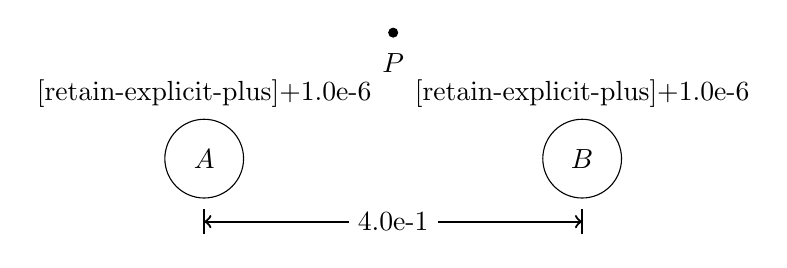
\begin{tikzpicture}[scale=0.8]
        %% Point P
        \draw[fill] (0,2) circle (2.0pt)
            node[anchor=north,yshift=-4pt] {$P$};
        %% Spheres A and B
        \draw[thick] (+3,-1.2) -- (+3,-0.8);
        \node[draw,circle,minimum size=1cm] at (-3,0) {$A$};
        \node[draw,circle,minimum size=1cm] at (+3,0) {$B$};
        \node[anchor=south] at (-3,0.66) {\SI[retain-explicit-plus]{+1.0e-6}{\coulomb}};
        \node[anchor=south] at (+3,0.66) {\SI[retain-explicit-plus]{+1.0e-6}{\coulomb}};
        %% Distance Label
        \draw[thick,<->] (-3,-1) -- (+3,-1)
            node[fill=white,pos=0.5,anchor=center] {\SI{4.0e-1}{\meter}};
        \draw[thick] (-3,-1.2) -- (-3,-0.8);
        \draw[thick] (+3,-1.2) -- (+3,-0.8);
    \end{tikzpicture}
}

\element{nysed}{
\begin{question}{Jan2008-Q43}
    Two small metallic spheres, $A$, and $B$, are separated by a distance \SI{4.0e-1}{\meter}, as shown.
    The charge on each sphere is \SI[retain-explicit-plus]{+1.0e-6}{\coulomb}.
    Point $P$ is located near the spheres.
    \begin{center}
        \JanTwoThousandEightQFortyThree
    \end{center}
    What is the magnitude of the electrostatic force between the two charges spheres?
    \begin{multicols}{2}
    \begin{choices}
        \wrongchoice{\SI{2.2e-2}{\newton}}
      \correctchoice{\SI{3.5e-2}{\newton}}
        \wrongchoice{\SI{2.2e4}{\newton}}
        \wrongchoice{\SI{5.6e4}{\newton}}
    \end{choices}
    \end{multicols}
\end{question}
}

\element{nysed}{
\begin{question}{Jan2008-Q44}
    Two small metallic spheres, $A$, and $B$, are separated by a distance \SI{4.0e-1}{\meter}, as shown.
    The charge on each sphere is \SI[retain-explicit-plus]{+1.0e-6}{\coulomb}.
    Point $P$ is located near the spheres.
    \begin{center}
        \JanTwoThousandEightQFortyThree
    \end{center}
    Which arrow best represents the direction of the resultant electric field at point $P$ due to the charges on spheres $A$ and $B$?
    \begin{multicols}{2}
    \begin{choices}
        \AMCboxDimensions{down=-0.8cm}
        \correctchoice{
            \begin{tikzpicture}[scale=2]
                \draw[dashed,white!60!black] (0,0) rectangle (1,1);
                \draw[thick,->] (0.5,0) -- (0.5,1);
            \end{tikzpicture}
        }
        \wrongchoice{
            \begin{tikzpicture}[scale=2]
                \draw[dashed,white!60!black] (0,0) rectangle (1,1);
                \draw[thick,->] (0,0.5) -- (1,0.5);
            \end{tikzpicture}
        }
        \wrongchoice{
            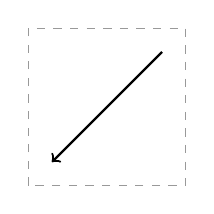
\begin{tikzpicture}[scale=2]
                \draw[dashed,white!60!black] (0,0) rectangle (1,1);
                \draw[thick,->] (0.85,0.85) -- (0.15,0.15);
            \end{tikzpicture}
        }
        \wrongchoice{
            \begin{tikzpicture}[scale=2]
                \draw[dashed,white!60!black] (0,0) rectangle (1,1);
                \draw[thick,->] (0.5,1) -- (0.5,0);
            \end{tikzpicture}
        }
    \end{choices}
    \end{multicols}
\end{question}
}


%% Section June2007
%%--------------------
\element{nysed}{
\begin{question}{June2007-Q15}
    If \SI{1}{\joule} of work is required to move \SI{1.0}{\coulomb} of charge between two points in an electric field,
        what is the potential difference between these points?
    \begin{multicols}{2}
    \begin{choices}
      \correctchoice{\SI{1.0e0}{\volt}}
        \wrongchoice{\SI{9.0e9}{\volt}}
        \wrongchoice{\SI{6.3e18}{\volt}}
        \wrongchoice{\SI{1.6e-19}{\volt}}
    \end{choices}
    \end{multicols}
\end{question}
}

\element{nysed}{
\begin{question}{June2007-Q32}
    Which quantity of excess electric charge could be found on an object?
    \begin{choices}
      \correctchoice{\SI{4.80e-19}{\coulomb}}
        \wrongchoice{\SI{6.25e-40}{\coulomb}}
        \wrongchoice{\num{6.25} elementary charges}
        \wrongchoice{\num{1.60} elementary charges}
    \end{choices}
\end{question}
}

\element{nysed}{
\begin{question}{June2007-Q33}
    The diagram below represents two electrically charged identical-sized metal spheres, $A$ and $B$.
    \begin{center}
    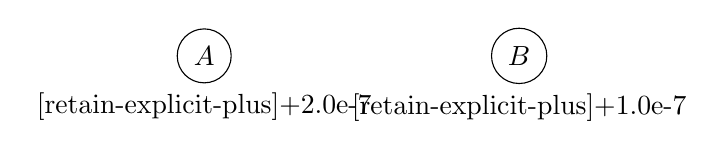
\begin{tikzpicture}
        \node[draw,circle,minimum size=0.5cm,anchor=center] (A) at (-2,0) {$A$};
        \node[anchor=north] at (A.south) {\SI[retain-explicit-plus]{+2.0e-7}{\coulomb}};
        \node[draw,circle,minimum size=0.5cm] (B) at (+2,0) {$B$};
        \node[anchor=north] at (B.south) {\SI[retain-explicit-plus]{+1.0e-7}{\coulomb}};
    \end{tikzpicture}
    \end{center}
    If the spheres are brought into contact,
        which sphere will have a net gain of electrons?
    \begin{multicols}{2}
    \begin{choices}
      \correctchoice{$A$, only}
        \wrongchoice{$B$, only}
        \wrongchoice{both $A$ and $B$}
        \wrongchoice{neither $A$ nor $B$}
    \end{choices}
    \end{multicols}
\end{question}
}


%% Section Jan2007
%%--------------------
\element{nysed}{
\begin{question}{Jan2007-Q01}
    Which is a vector quantity?
    \begin{choices}
        \wrongchoice{electric charge}
      \correctchoice{electric field strength}
        \wrongchoice{electric potential difference}
        \wrongchoice{electric resistance}
    \end{choices}
\end{question}
}

\element{nysed}{
\begin{question}{Jan2007-Q15}
    If \SI{60}{\joule} of work is required to move \SI{5.0}{\coulomb} of charge between two points in an electric field, what is the potential difference between these points?
    \begin{multicols}{2}
    \begin{choices}
      \correctchoice{\SI{12}{\volt}}
        \wrongchoice{\SI{5.0}{\volt}}
        \wrongchoice{\SI{60}{\volt}}
        \wrongchoice{\SI{300}{\volt}}
    \end{choices}
    \end{multicols}
\end{question}
}

\element{nysed}{
\begin{question}{Jan2007-Q18}
    If the distance separating an electron and a proton is halved,
        the magnitude of the electrostatic force, between these charged particles will be:
    \begin{multicols}{2}
    \begin{choices}
      \correctchoice{quadrupled}
        \wrongchoice{doubled}
        \wrongchoice{unchanged}
        \wrongchoice{quartered}
    \end{choices}
    \end{multicols}
\end{question}
}

\element{nysed}{
\begin{question}{Jan2007-Q19}
    Two similar metal spheres, $A$ and $B$, have charges of \SI[retain-explicit-plus]{+2.0e-6}{\coulomb} and \SI[retain-explicit-plus]{+1.0e-6}{\coulomb},
        respectively, as shown in the diagram below.
    \begin{center}
    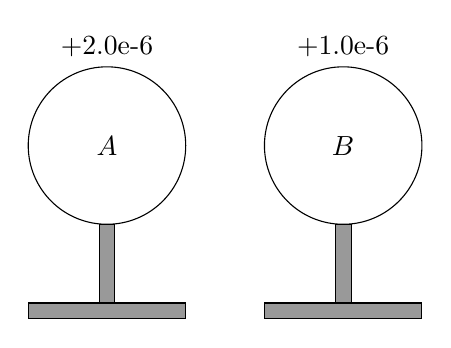
\begin{tikzpicture}
        \begin{scope}[xshift=-1.5cm]
            \draw (0,0) circle (1cm);
            \node[anchor=center] at (0,0) {$A$};
            \node[anchor=south] at (0,1) {\SI{+2.0e-6}{\coulomb}};
            \draw[fill=white!60!black] (-0.1,-1) rectangle (0.1,-2);
            \draw[fill=white!60!black] (-1,-2) rectangle (1,-2.2);
        \end{scope}
        \begin{scope}[xshift=+1.5cm]
            \draw (0,0) circle (1cm);
            \node[anchor=center] at (0,0) {$B$};
            \node[anchor=south] at (0,1) {\SI{+1.0e-6}{\coulomb}};
            \draw[fill=white!60!black] (-0.1,-1) rectangle (0.1,-2);
            \draw[fill=white!60!black] (-1,-2) rectangle (1,-2.2);
        \end{scope}
    \end{tikzpicture}
    \end{center}
    The magnitude of the electrostatic force on $A$ due to $B$ is \SI{2.4}{\newton}.
    What is the magnitude of the electrostatic force on $B$ due to $A$?
    \begin{multicols}{2}
    \begin{choices}
      \correctchoice{\SI{2.4}{\newton}}
        \wrongchoice{\SI{1.2}{\newton}}
        \wrongchoice{\SI{4.8}{\newton}}
        \wrongchoice{\SI{9.6}{\newton}}
    \end{choices}
    \end{multicols}
\end{question}
}

\element{nysed}{
\begin{question}{Jan2007-Q20}
    In the diagram below, $P$ is a point near a negatively charged sphere.
    \begin{center}
    \begin{tikzpicture}
        %% charge
        \draw[thick] (-0.5ex,0) -- (0.5ex,0);
        \draw (0,0) circle (1ex);
        %% point P
        \fill (2,0) circle (2pt) node[anchor=west] {$P$};
    \end{tikzpicture}
    \end{center}
    Which vector best represent the direction of the electric field at point $P$?
    \begin{multicols}{2}
    \begin{choices}
        \AMCboxDimensions{down=-0.8cm}
        \correctchoice{
            \begin{tikzpicture}[scale=2]
                \draw[dashed,white!60!black] (0,0) rectangle (1,1);
                \draw[thick,->] (1,0.5) -- (0,0.5);
            \end{tikzpicture}
        }
        \wrongchoice{
            \begin{tikzpicture}[scale=2]
                \draw[dashed,white!60!black] (0,0) rectangle (1,1);
                \draw[thick,->] (0,0.5) -- (1,0.5);
            \end{tikzpicture}
        }
        \wrongchoice{
            \begin{tikzpicture}[scale=2]
                \draw[dashed,white!60!black] (0,0) rectangle (1,1);
                \draw[thick,->] (0.5,0) -- (0.5,1);
            \end{tikzpicture}
        }
        \wrongchoice{
            \begin{tikzpicture}[scale=2]
                \draw[dashed,white!60!black] (0,0) rectangle (1,1);
                \draw[thick,->] (0.5,1) -- (0.5,0);
            \end{tikzpicture}
        }
    \end{choices}
    \end{multicols}
\end{question}
}

\element{nysed}{
\begin{question}{Jan2007-Q31}
    Metal sphere $A$ has a charge of \num{-2} units and an identical metal sphere, $B$, has a charge of \num{-4} units.
    If the spheres are brought into contact with each other and then separated, the charge on sphere $B$ will be
    \begin{multicols}{2}
    \begin{choices}
      \correctchoice{\num{-3} units}
        \wrongchoice{\num{0} units}
        \wrongchoice{\num[retain-explicit-plus]{+4} units}
        \wrongchoice{\num{-3} units}
    \end{choices}
    \end{multicols}
\end{question}
}

\element{nysed}{
\begin{question}{Jan2007-Q33}
    What is the net electrical charge on a magnesium ion that is formed when a neutral magnesium atom loses two electrons?
    \begin{multicols}{2}
    \begin{choices}
        \wrongchoice{\SI[retain-explicit-plus]{-3.2e-19}{\coulomb}}
        \wrongchoice{\SI[retain-explicit-plus]{-1.6e-19}{\coulomb}}
        \wrongchoice{\SI[retain-explicit-plus]{+1.6e-19}{\coulomb}}
      \correctchoice{\SI[retain-explicit-plus]{+3.2e-19}{\coulomb}}
    \end{choices}
    \end{multicols}
\end{question}
}

\element{nysed}{
\begin{question}{Jan2007-Q47}
    Which quantity and unit are correctly paired?
    \begin{choices}
      \correctchoice{electric field strength and \si{\newton\per\coulomb}}
        \wrongchoice{current and \si{\coulomb\second}}
        \wrongchoice{potential difference and \si{\eV}}
        \wrongchoice{resistivity and \si{\ohm\per\meter}}
    \end{choices}
\end{question}
}


%% Section June2006
%%--------------------
\element{nysed}{
\begin{question}{June2006-Q10}
    A positively charged glass rod attracts object $X$.
    The net charge of object $X$
    \begin{choices}
      \correctchoice{may be zero or negative}
        \wrongchoice{may be zero or positive}
        \wrongchoice{must be positive}
        \wrongchoice{must be negative}
    \end{choices}
\end{question}
}

\element{nysed}{
\begin{question}{June2006-Q42}
    What is the magnitude of the electric field intensity at a point where a proton experiences an electrostatic force of magnitude \SI{2.3e-25}{\newton}?
    \begin{multicols}{2}
    \begin{choices}
      \correctchoice{\SI{1.44e-6}{\newton\per\coulomb}}
        \wrongchoice{\SI{1.44e44}{\newton\per\coulomb}}
        \wrongchoice{\SI{3.68e-44}{\newton\per\coulomb}}
        \wrongchoice{\SI{3.68e6}{\newton\per\coulomb}}
    \end{choices}
    \end{multicols}
\end{question}
}

\element{nysed}{
\begin{question}{June2006-Q47}
    Which graph best represents the relationship between the strength of an electric field and distance from a point charge?
    \begin{multicols}{2}
    \begin{choices}
        \AMCboxDimensions{down=-2.5em}
        \correctchoice{
            \begin{tikzpicture}
                \begin{axis}[
                    axis y line=left,
                    axis x line=bottom,
                    axis line style={->},
                    xlabel={distance},
                    xtick=\empty,
                    ylabel={electric field},
                    ytick=\empty,
                    xmin=0,xmax=11,
                    ymin=0,ymax=11,
                    width=\columnwidth,
                    very thin,
                ]
                \addplot[line width=1pt,domain=0:10]{10/x^2};
                \end{axis}
            \end{tikzpicture}
        }
        \wrongchoice{
            \begin{tikzpicture}
                \begin{axis}[
                    axis y line=left,
                    axis x line=bottom,
                    axis line style={->},
                    xlabel={distance},
                    xtick=\empty,
                    ylabel={electric field},
                    ytick=\empty,
                    xmin=0,xmax=11,
                    ymin=0,ymax=11,
                    width=\columnwidth,
                    very thin,
                ]
                \addplot[line width=1pt,domain=0:10]{0.1*x*x};
                \end{axis}
            \end{tikzpicture}
        }
        \wrongchoice{
            \begin{tikzpicture}
                \begin{axis}[
                    axis y line=left,
                    axis x line=bottom,
                    axis line style={->},
                    xlabel={distance},
                    xtick=\empty,
                    ylabel={electric field},
                    ytick=\empty,
                    xmin=0,xmax=11,
                    ymin=0,ymax=11,
                    width=\columnwidth,
                    very thin,
                ]
                \addplot[line width=1pt,domain=0:10]{8};
                \end{axis}
            \end{tikzpicture}
        }
        \wrongchoice{
            \begin{tikzpicture}
                \begin{axis}[
                    axis y line=left,
                    axis x line=bottom,
                    axis line style={->},
                    xlabel={distance},
                    xtick=\empty,
                    ylabel={electric field},
                    ytick=\empty,
                    xmin=0,xmax=11,
                    ymin=0,ymax=11,
                    width=\columnwidth,
                    very thin,
                ]
                \addplot[line width=1pt,domain=0:10]{x};
                \end{axis}
            \end{tikzpicture}
        }
    \end{choices}
    \end{multicols}
\end{question}
}


%% Section Jan2006
%%--------------------
\element{nysed}{
\begin{question}{Jan2006-Q24}
    How much electrical energy is required to move a \SI{4.00}{\micro\coulomb} charge through a potential difference of \SI{36.0}{\volt}?
    \begin{multicols}{2}
    \begin{choices}
        \wrongchoice{\SI{9.00e6}{\joule}}
        \wrongchoice{\SI{1.44}{\joule}}
      \correctchoice{\SI{1.44e-4}{\joule}}
        \wrongchoice{\SI{1.11e-7}{\joule}}
    \end{choices}
    \end{multicols}
\end{question}
}

\element{nysed}{
\begin{question}{Jan2006-Q27}
    An electron placed between oppositely charged parallel plates $A$ and $B$ moves toward plate $A$, as represented in the diagram below.
    \begin{center}
    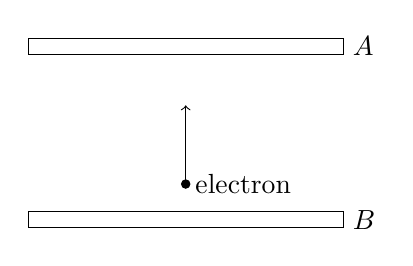
\begin{tikzpicture}
        %% Top A
        \draw (-2,2) rectangle (2,2.2);
        \node[anchor=west] at (2,2.1) {$A$};
        %% Bottom B
        \draw (-2,0) rectangle (2,-0.2);
        \node[anchor=west] at (2,-0.1) {$B$};
        %% Electron
        \draw[fill] (0,1em) circle (1.5pt)
            node[anchor=west] {electron};
        \draw[->] (0,1em) -- ++(90:1cm);
    \end{tikzpicture}
    \end{center}
    What is the direction of the electric field between the plates?
    \begin{multicols}{2}
    \begin{choices}
      \correctchoice{toward plate $B$}
        \wrongchoice{toward plate $A$}
        \wrongchoice{into the page}
        \wrongchoice{out of the page}
    \end{choices}
    \end{multicols}
\end{question}
}

\element{nysed}{
\begin{question}{Jan2006-Q33}
    Oil droplets may gain electrical charges as they are produced through a nozzle.
    Which quantity of charge is \emph{not} possible on an oil droplet?
    \begin{multicols}{2}
    \begin{choices}
      \correctchoice{\SI{4.8e-19}{\coulomb}}
        \wrongchoice{\SI{8.0e-19}{\coulomb}}
        \wrongchoice{\SI{3.2e-19}{\coulomb}}
        \wrongchoice{\SI{2.6e-19}{\coulomb}}
    \end{choices}
    \end{multicols}
\end{question}
}


%% Section June2005
%%--------------------
\element{nysed}{
\begin{question}{June2005-Q14}
    Two positively charged masses are separated by a distance $r$.
    Which statement best describes the gravitational and electrostatic forces between the two masses?
    \begin{choices}
      \correctchoice{the gravitational force is attractive and the electrostatic force is repulsive.}
        \wrongchoice{the gravitational force is attractive and the electrostatic force is attractive.}
        \wrongchoice{Both forces are attractive.}
        \wrongchoice{Both forces are repulsive.}
    \end{choices}
\end{question}
}

\element{nysed}{
\begin{question}{June2005-Q31}
    A metal sphere has a net negative charge of \SI{1.1e-6}{\coulomb}.
    Approximately how many more electrons than protons are on the sphere?
    \begin{multicols}{2}
    \begin{choices}
      \correctchoice{\num{6.9e12}}
        \wrongchoice{\num{1.8e12}}
        \wrongchoice{\num{5.7e12}}
        \wrongchoice{\num{9.9e12}}
    \end{choices}
    \end{multicols}
\end{question}
}

\element{nysed}{
\begin{question}{June2005-Q37}
    Which physical quantity is correctly paired with its unit?
    \begin{choices}
      \correctchoice{electric potential and \si{\joule\per\coulomb}}
        \wrongchoice{power and \si{\watt\second}}
        \wrongchoice{energy and \si{\newton\second}}
        \wrongchoice{electric current and \si{\ampere\per\coulomb}}
    \end{choices}
\end{question}
}

\element{nysed}{
\begin{question}{June2005-Q47}
    Which graph best represents the relationship between the magnitude of the electrostatic force and the distance between two oppositely charged particles?
    \begin{multicols}{2}
    \begin{choices}
        \AMCboxDimensions{down=-2.5em}
        \correctchoice{
            \begin{tikzpicture}
                \begin{axis}[
                    axis y line=left,
                    axis x line=bottom,
                    axis line style={->},
                    xlabel={distance},
                    xtick=\empty,
                    ylabel={force},
                    ytick=\empty,
                    xmin=0,xmax=11,
                    ymin=0,ymax=11,
                    width=\columnwidth,
                    very thin,
                ]
                \addplot[line width=1pt,domain=0:10]{10/x^2};
                \end{axis}
            \end{tikzpicture}
        }
        \wrongchoice{
            \begin{tikzpicture}
                \begin{axis}[
                    axis y line=left,
                    axis x line=bottom,
                    axis line style={->},
                    xlabel={distance},
                    xtick=\empty,
                    ylabel={force},
                    ytick=\empty,
                    xmin=0,xmax=11,
                    ymin=0,ymax=11,
                    width=\columnwidth,
                    very thin,
                ]
                \addplot[line width=1pt,domain=0:10]{0.1*x*x};
                \end{axis}
            \end{tikzpicture}
        }
        \wrongchoice{
            \begin{tikzpicture}
                \begin{axis}[
                    axis y line=left,
                    axis x line=bottom,
                    axis line style={->},
                    xlabel={distance},
                    xtick=\empty,
                    ylabel={force},
                    ytick=\empty,
                    xmin=0,xmax=11,
                    ymin=0,ymax=11,
                    width=\columnwidth,
                    very thin,
                ]
                \addplot[line width=1pt,domain=0:10]{8};
                \end{axis}
            \end{tikzpicture}
        }
        \wrongchoice{
            \begin{tikzpicture}
                \begin{axis}[
                    axis y line=left,
                    axis x line=bottom,
                    axis line style={->},
                    xlabel={distance},
                    xtick=\empty,
                    ylabel={force},
                    ytick=\empty,
                    xmin=0,xmax=11,
                    ymin=0,ymax=11,
                    width=\columnwidth,
                    very thin,
                ]
                \addplot[line width=1pt,domain=0:10]{x};
                \end{axis}
            \end{tikzpicture}
        }
    \end{choices}
    \end{multicols}
\end{question}
}


%% Section Jan2005
%%--------------------
\element{nysed}{
\begin{question}{Jan2005-Q25}
    In an electric field, \SI{0.90}{\joule} of work is required to bring \SI{0.45}{\coulomb} of charge from point $A$ to point $B$.
    What is the electric potential difference between points $A$ and $B$?
    \begin{multicols}{2}
    \begin{choices}
      \correctchoice{\SI{2.0}{\volt}}
        \wrongchoice{\SI{5.0}{\volt}}
        \wrongchoice{\SI{0.50}{\volt}}
        \wrongchoice{\SI{0.41}{\volt}}
    \end{choices}
    \end{multicols}
\end{question}
}

\element{nysed}{
\begin{question}{Jan2005-Q32}
    In the diagram below, proton $p$, neutron $n$, and electron $e$ are located as shown between two oppositely charged plates.
    \begin{center}
    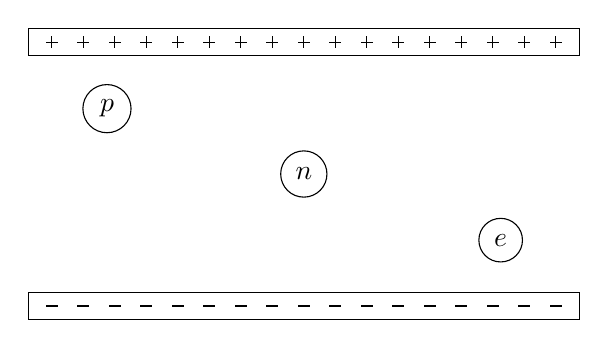
\begin{tikzpicture}
        %% Bottom
        \draw (0,0) rectangle (7,-1em);
        \foreach \x in {3,7,...,69} {
            \draw (\x mm,-0.5em) -- ++(0:0.5ex);
            \draw (\x mm,-0.5em) -- ++(180:0.5ex);
        }
        %% Top
        \draw (0,3) rectangle (7,3cm+1em);
        \foreach \x in {3,7,...,69} {
            \draw (\x mm,3cm+0.5em) -- ++(0:0.5ex);
            \draw (\x mm,3cm+0.5em) -- ++(180:0.5ex);
            \draw (\x mm,3cm+0.5em) -- ++(90:0.5ex);
            \draw (\x mm,3cm+0.5em) -- ++(270:0.5ex);
        }
        %% Proton, Neutron, Electron
        \node[draw,anchor=center,circle] at (1.0,2.33) {$p$};
        \node[draw,anchor=center,circle] at (3.5,1.50) {$n$};
        \node[draw,anchor=center,circle] at (6.0,0.66) {$e$};
    \end{tikzpicture}
    \end{center}
    The magnitude of acceleration will be greatest for the:
    \begin{choices}
      \correctchoice{electron, because it has the smallest mass}
        \wrongchoice{proton, because it is farthest from the negative plate}
        \wrongchoice{neutron, because it is neutral}
        \wrongchoice{neutron, because it has the greatest mass}
    \end{choices}
\end{question}
}

\element{nysed}{
\begin{question}{Jan2005-Q33}
    Two protons are located one meter apart.
    Compared to the gravitational force of attraction between the two protons,
        the electrostatic force between the protons is:
    \begin{choices}
      \correctchoice{stronger and repulsive}
        \wrongchoice{weaker and repulsive}
        \wrongchoice{stronger and attractive}
        \wrongchoice{weaker and attractive}
    \end{choices}
\end{question}
}

\element{nysed}{
\begin{question}{Jan2005-Q35}
    A balloon is rubbed against a student's hair and then touched to a wall.
    The balloon ``sticks'' to the wall due to:
    \begin{choices}
      \correctchoice{electrostatic forces between the particles of the balloon and the particles of the wall}
        \wrongchoice{electrostatic forces between the particles of the balloon}
        \wrongchoice{magnetic forces between the particles of the wall}
        \wrongchoice{magnetic forces between the particles of the balloon and the particles of the wall}
    \end{choices}
\end{question}
}

\element{nysed}{
\begin{question}{Jan2005-Q40}
    In the diagram below, a positive test charge is located between two charged spheres, $A$ and $B$.
    Sphere $A$ has a charge of $+2q$ and is located \SI{0.2}{\meter} from the test charge.
    Sphere $B$ has a charge of $-2q$ and is located \SI{0.1}{\meter} from the test charge.
    \begin{center}
    \begin{tikzpicture}[scale=1.2]
        %% coordinates
        \coordinate (A) at (-4,0);
        \coordinate (T) at (0,0);
        \coordinate (B) at (2,0);
        %% charge A
        \draw[dashed] (A) -- ++(270:2);
        \node[anchor=center,draw,circle,fill=white,circle] at (A) {$+2q$};
        %% charge B
        \draw[dashed] (B) -- ++(270:2);
        \node[anchor=center,draw,circle,fill=white,circle] at (B) {$-2q$};
        %% test charge
        \draw[dashed] (T) -- ++(270:2);
        \draw[fill=white] (T) circle (1ex);
        \foreach \x in {0,90,180,270} \draw[thick] (T) -- ++(\x:0.5ex);
        \node[pin={[pin edge={latex-}]135:Test charge},shift={(135:1ex)}] at (T) {};
        %% distance labels
        \draw[<->] (A) ++ (270:1.33) -- ++(0:4) node[pos=0.5,anchor=center,fill=white] {\SI{0.2}{\meter}};
        \draw[<->] (B) ++ (270:1.33) -- ++(180:2) node[pos=0.5,anchor=center,fill=white] {\SI{0.1}{\meter}};
    \end{tikzpicture}
    \end{center}
    If the magnitude of the force on the test charge due to sphere $B$ is $F$,
        what is the magnitude of the force on the test charge due to sphere $B$?
    \begin{multicols}{4}
    \begin{choices}
      \correctchoice{$4F$}
        \wrongchoice{$2F$}
        \wrongchoice{$\dfrac{F}{4}$}
        \wrongchoice{$\dfrac{F}{2}$}
    \end{choices}
    \end{multicols}
\end{question}
}


%% Section June2004
%%--------------------
\element{nysed}{
\begin{question}{June2004-Q17}
    A negatively charged plastic comb is brought close to,
        but does not touch, a small piece of paper.
    If the comb and the paper are attracted to each other,
        the charge on the paper
    \begin{choices}
      \correctchoice{may be positive or neutral}
        \wrongchoice{may be negative or neutral}
        \wrongchoice{must be negative}
        \wrongchoice{must be positive}
    \end{choices}
\end{question}
}

\element{nysed}{
\begin{question}{June2004-Q18}
    If a \SI{1.5}{\volt} cell is to be completely recharged each electron must be supplied with a minimum energy of
    \begin{multicols}{2}
    \begin{choices}
      \correctchoice{\SI{1.5}{\eV}}
        \wrongchoice{\SI{9.5e18}{\eV}}
        \wrongchoice{\SI{1.5}{\joule}}
        \wrongchoice{\SI{9.5e18}{\joule}}
    \end{choices}
    \end{multicols}
\end{question}
}

\element{nysed}{
\begin{question}{June2004-Q20}
    A moving electron is deflected by two oppositely charged parallel plates,
        as shown in the diagram below.
    \begin{center}
    \begin{tikzpicture}
        %% NOTE: TODO: draw
        %% electron
    \end{tikzpicture}
    \includegraphics[keepaspectratio,width=\linewidth]{June2004-Q20}
    \end{center}
    The electric field between the plates is directed from
    \begin{multicols}{2}
    \begin{choices}
        \wrongchoice{$A$ to $B$}
        \wrongchoice{$B$ to $A$}
      \correctchoice{$C$ to $D$}
        \wrongchoice{$D$ to $C$}
    \end{choices}
    \end{multicols}
\end{question}
}

\element{nysed}{
\begin{question}{June2004-Q21}
    The diagram below shows two identical metal spheres,
        $A$ and $B$, separated by a distance $d$.
    Each sphere has mass $m$ and posses charge $+q$.
    %% NOTE: close duplicate of June2003-Q41
    \begin{center}
    \begin{tikzpicture}
        \node[draw,circle,anchor=center] (A) at (0,0) {$A$};
        \node[draw,circle,anchor=center] (B) at (4,0) {$B$};
        \draw[dashed] (A) -- (0,1.5);
        \draw[dashed] (B) -- (4,1.5);
        \draw[<->] (0,1.0) -- (4,1.0) node[fill=white,pos=0.5,anchor=center] {$d$};
    \end{tikzpicture}
    \end{center}
    Which diagram best represents the electrostatic force $F_e$ and the gravitational force $F_g$ acting on sphere $B$ due to sphere $A$?
    [Vectors are not drawn to scale]
    \begin{multicols}{2}
    \begin{choices}
        \AMCboxDimensions{down=-2.5em}
        \correctchoice{
            \begin{tikzpicture}
                \draw[white] (-1.6,-2.5em) rectangle (1.6,2.5em);
                \node[draw,circle,anchor=center] (A) at (0,0) {$B$};
                \draw[->] (A) -- ++(0:1.5) node[anchor=south east] {$F_e$};
                \draw[->] (A) -- ++(180:1.0) node[anchor=south west] {$F_g$};
            \end{tikzpicture}
        }
        \wrongchoice{
            \begin{tikzpicture}
                \draw[white] (-1.6,-2.5em) rectangle (1.6,2.5em);
                \node[draw,circle,anchor=center] (A) at (0,0) {$B$};
                \draw[->] (A) -- ++(180:1.5) node[anchor=south west] {$F_e$};
                \draw[->] (A) -- ++(0:1.0) node[anchor=south east] {$F_g$};
            \end{tikzpicture}
        }
        \wrongchoice{
            \begin{tikzpicture}
                \draw[white] (-1.6,-2.5em) rectangle (1.6,2.5em);
                \node[draw,circle,anchor=center] (A) at (0,0) {$B$};
                \draw[->] (A.north east) -- ++(0:1.5) node[anchor=south east] {$F_e$};
                \draw[->] (A.south east) -- ++(0:1.0) node[anchor=north east] {$F_g$};
            \end{tikzpicture}
        }
        \wrongchoice{
            \begin{tikzpicture}
                \draw[white] (-1.6,-2.5em) rectangle (1.6,2.5em);
                \node[draw,circle,anchor=center] (A) at (0,0) {$B$};
                \draw[->] (A.north west) -- ++(180:1.5) node[anchor=south west] {$F_e$};
                \draw[->] (A.south west) -- ++(180:1.0) node[anchor=north west] {$F_g$};
            \end{tikzpicture}
        }
    \end{choices}
    \end{multicols}
\end{question}
}

\element{nysed}{
\begin{question}{June2004-Q45}
    Which graph best represents the relationship between the magnitude of the electric field strength around a point charge and the distance from the point charge?
    \begin{multicols}{2}
    \begin{choices}
        \AMCboxDimensions{down=-2.5em}
        \correctchoice{
            \begin{tikzpicture}
                \begin{axis}[
                    axis y line=left,
                    axis x line=bottom,
                    axis line style={->},
                    xlabel={distance},
                    xtick=\empty,
                    ylabel={electric field},
                    ytick=\empty,
                    xmin=0,xmax=11,
                    ymin=0,ymax=11,
                    width=\columnwidth,
                    very thin,
                ]
                \addplot[line width=1pt,domain=0:10]{10/x^2};
                \end{axis}
            \end{tikzpicture}
        }
        \wrongchoice{
            \begin{tikzpicture}
                \begin{axis}[
                    axis y line=left,
                    axis x line=bottom,
                    axis line style={->},
                    xlabel={distance},
                    xtick=\empty,
                    ylabel={electric field},
                    ytick=\empty,
                    xmin=0,xmax=11,
                    ymin=0,ymax=11,
                    width=\columnwidth,
                    very thin,
                ]
                \addplot[line width=1pt,domain=0:10]{0.1*x*x};
                \end{axis}
            \end{tikzpicture}
        }
        \wrongchoice{
            \begin{tikzpicture}
                \begin{axis}[
                    axis y line=left,
                    axis x line=bottom,
                    axis line style={->},
                    xlabel={distance},
                    xtick=\empty,
                    ylabel={electric field},
                    ytick=\empty,
                    xmin=0,xmax=11,
                    ymin=0,ymax=11,
                    width=\columnwidth,
                    very thin,
                ]
                \addplot[line width=1pt,domain=0:10]{10-x};
                \end{axis}
            \end{tikzpicture}
        }
        \wrongchoice{
            \begin{tikzpicture}
                \begin{axis}[
                    axis y line=left,
                    axis x line=bottom,
                    axis line style={->},
                    xlabel={distance},
                    xtick=\empty,
                    ylabel={electric field},
                    ytick=\empty,
                    xmin=0,xmax=11,
                    ymin=0,ymax=11,
                    width=\columnwidth,
                    very thin,
                ]
                \addplot[line width=1pt,domain=0:10]{x};
                \end{axis}
            \end{tikzpicture}
        }
    \end{choices}
    \end{multicols}
\end{question}
}


%% Section Jan2004
%%--------------------
\element{nysed}{
\begin{question}{Jan2004-Q09}
    The diagram below shows two small metal spheres, $A$ and $B$.
    Each sphere possesses a net charge of \SI{4.0e-6}{\coulomb}.
    The spheres are separated by a distance of \SI{1.0}{\meter}.
    \begin{center}
    \begin{tikzpicture}
        \coordinate (A) at (-1.5,0);
        \coordinate (B) at (+1.5,0);
        %% point A
        \fill (A) circle (2pt);
        \node[anchor=south] at (A)  {\SI{4.0e-6}{\coulomb}};
        \node[anchor=north] at (A)  {$A$};
        %% point B
        \fill (B) circle (2pt);
        \node[anchor=south] at (B)  {\SI{4.0e-6}{\coulomb}};
        \node[anchor=north] at (B)  {$B$};
        %% distance
        \draw[thick,<->,shorten <=1mm,shorten >=1mm] (A) -- (B) node[pos=0.5,anchor=north] {\SI{1.0}{\meter}};
    \end{tikzpicture}
    \end{center}
    Which combination of charged spheres and separation distance produces an electrostatic force of the same magnitude as the electrostatic force between spheres $A$ and $B$?
    \begin{choices}
        \AMCboxDimensions{down=-0.4cm}
        \wrongchoice{
            \begin{tikzpicture}
                \draw[dashed,white!60!black] (-3.5,-0.75) rectangle (3.5,0.75);
                \coordinate (A) at (-0.6,0);
                \coordinate (B) at (+0.6,0);
                %% point A
                \fill (A) circle (2pt);
                \node[anchor=east] at (A)  {\SI{2.0e-6}{\coulomb}};
                \node[anchor=north] at (A)  {$A$};
                %% point B
                \fill (B) circle (2pt);
                \node[anchor=west] at (B)  {\SI{2.0e-6}{\coulomb}};
                \node[anchor=north] at (B)  {$B$};
                %% distance
                \draw[thick,<->,shorten <=1mm,shorten >=1mm] (A) -- (B) node[pos=0.5,anchor=south] {\SI{0.40}{\meter}};
            \end{tikzpicture}
        }
        \wrongchoice{
            \begin{tikzpicture}
                \draw[dashed,white!60!black] (-3.5,-0.75) rectangle (3.5,0.75);
                \coordinate (A) at (-1.2,0);
                \coordinate (B) at (+1.2,0);
                %% point A
                \fill (A) circle (2pt);
                \node[anchor=south east] at (A)  {\SI{6.0e-6}{\coulomb}};
                \node[anchor=north] at (A)  {$A$};
                %% point B
                \fill (B) circle (2pt);
                \node[anchor=south west] at (B)  {\SI{4.0e-6}{\coulomb}};
                \node[anchor=north] at (B)  {$B$};
                %% distance
                \draw[thick,<->,shorten <=1mm,shorten >=1mm] (A) -- (B) node[pos=0.5,anchor=center,fill=white] {\SI{0.80}{\meter}};
            \end{tikzpicture}
        }
        \wrongchoice{
            \begin{tikzpicture}
                \draw[dashed,white!60!black] (-3.5,-0.75) rectangle (3.5,0.75);
                \coordinate (A) at (-2.4,0);
                \coordinate (B) at (+2.4,0);
                %% point A
                \fill (A) circle (2pt);
                \node[anchor=south] at (A)  {\SI{8.0e-6}{\coulomb}};
                \node[anchor=north] at (A)  {$A$};
                %% point B
                \fill (B) circle (2pt);
                \node[anchor=south] at (B)  {\SI{4.0e-6}{\coulomb}};
                \node[anchor=north] at (B)  {$B$};
                %% distance
                \draw[thick,<->,shorten <=1mm,shorten >=1mm] (A) -- (B) node[pos=0.5,anchor=center,fill=white] {\SI{1.6}{\meter}};
            \end{tikzpicture}
        }
        \correctchoice{
            \begin{tikzpicture}
                \draw[dashed,white!60!black] (-3.5,-0.75) rectangle (3.5,0.75);
                \coordinate (A) at (-3,0);
                \coordinate (B) at (+3,0);
                %% point A
                \fill (A) circle (2pt);
                \node[anchor=south west] at (A)  {\SI{8.0e-6}{\coulomb}};
                \node[anchor=north] at (A)  {$A$};
                %% point B
                \fill (B) circle (2pt);
                \node[anchor=south east] at (B)  {\SI{8.0e-6}{\coulomb}};
                \node[anchor=north] at (B)  {$B$};
                %% distance
                \draw[thick,<->,shorten <=1mm,shorten >=1mm] (A) -- (B) node[pos=0.5,anchor=center,fill=white] {\SI{2.0}{\meter}};
            \end{tikzpicture}
        }
    \end{choices}
\end{question}
}

\element{nysed}{
\begin{question}{Jan2004-Q13}
    A positive test charge is placed between an electron, $e$,
        and a proton, $p$, as shown in the diagram below.
    \begin{center}
    \begin{tikzpicture}
        %% proton and electron
        \node[anchor=center,circle,draw] (D) at (-2,0) {$e$};
        \node[anchor=center,circle,draw] (B) at (+2,0) {$p$};
        \node[anchor=center] (A) at (0,+1.5) {$A$};
        \node[anchor=center] (C) at (0,-1.5) {$C$};
        \node[anchor=west] at (D.east) {$D$};
        \node[anchor=east] at (B.west) {$B$};
        %% test charge
        \foreach \x in {0,90,180,270}
            \draw[thick] (0,0) -- (\x:0.5ex);
        \draw[thick] (0,0) circle (1ex);
        \node[pin={[pin edge={latex-}]50:Test charge}] at (45:1ex) {};
    \end{tikzpicture}
    \end{center}
    When the test charge is released, it will move toward:
    \begin{multicols}{4}
    \begin{choices}[o]
        \wrongchoice{$A$}
        \wrongchoice{$B$}
        \wrongchoice{$C$}
      \correctchoice{$D$}
    \end{choices}
    \end{multicols}
\end{question}
}


%% Section June2003
%%--------------------
\element{nysed}{
\begin{question}{June2003-Q17}
    The magnitude of the electrostatic force between two point charges is $F$.
    If the distance between the charges is doubled,
        the electrostatic force between the charges will become.
    \begin{multicols}{4}
    \begin{choices}
      \correctchoice{$\dfrac{F}{4}$}
        \wrongchoice{$2F$}
        \wrongchoice{$\dfrac{F}{2}$}
        \wrongchoice{$4F$}
    \end{choices}
    \end{multicols}
\end{question}
}

\element{nysed}{
\begin{question}{June2003-Q21}
    If \SI{4.8e-17}{\joule} of work is required to move an electron between two points in an electric field,
        what is the electric potential difference between these points?
    \begin{multicols}{2}
    \begin{choices}
      \correctchoice{\SI{3.0e2}{\volt}}
        \wrongchoice{\SI{1.6e-19}{\volt}}
        \wrongchoice{\SI{4.8e2}{\volt}}
        \wrongchoice{\SI{4.8e-17}{\volt}}
    \end{choices}
    \end{multicols}
\end{question}
}

\element{nysed}{
\begin{question}{June2003-Q37}
    An object with a net charge of \SI{4.80e-6}{\coulomb} experiences an electrostatic force having a magnitude of \SI{6.00e-2}{\newton} when placed near a negatively charged metal sphere.
    What is the electric field strength at this location?
    \begin{choices}
      \correctchoice{\SI{1.25e4}{\newton\per\coulomb} directed toward the sphere}
        \wrongchoice{\SI{1.25e4}{\newton\per\coulomb} directed away from the sphere}
        \wrongchoice{\SI{2.88e-8}{\newton\per\coulomb} directed away from the sphere}
        \wrongchoice{\SI{2.88e-8}{\newton\per\coulomb} directed toward the sphere}
    \end{choices}
\end{question}
}

\element{nysed}{
\begin{question}{June2003-Q41}
    In the diagram below, two positively charged spheres, $A$ and $B$,
        of masses $m_a$ and $m_b$ are located a distance $d$ apart.
    %% NOTE: close duplicate of June2004-Q21
    \begin{center}
    \begin{tikzpicture}
        \node[draw,circle,anchor=center] (A) at (0,0) {$A$};
        \node[draw,circle,anchor=center,minimum size=1.5cm] (B) at (4,0) {$B$};
        \draw[dashed] (A) -- (0,2);
        \draw[dashed] (B) -- (4,2);
        \draw[<->] (0,1.5) -- (4,1.5)
            node[pos=0.5,anchor=south] {$d$};
    \end{tikzpicture}
    \end{center}
    Which diagram best represents the directions of the gravitational force,
        $F_g$, and the electrostatic force, $F_e$, acting on sphere $A$ due to the mass and charge of sphere $B$?
    Vectors are not drawn to scale.
    \begin{multicols}{2}
    \begin{choices}
        \AMCboxDimensions{down=-1.25em}
        \correctchoice{
            \begin{tikzpicture}
                \draw[white] (-1.6,-2.5em) rectangle (1.6,2.5em);
                \node[draw,circle,anchor=center] (A) at (0,0) {$A$};
                \draw[->] (A) -- ++(180:1.5)
                    node[anchor=south west] {$F_e$};
                \draw[->] (A) -- ++(0:1.0)
                    node[anchor=south east] {$F_g$};
            \end{tikzpicture}
        }
        \wrongchoice{
            \begin{tikzpicture}
                \draw[white] (-1.6,-2.5em) rectangle (1.6,2.5em);
                \node[draw,circle,anchor=center] (A) at (0,0) {$A$};
                \draw[->] (A) -- ++(0:1.5)
                    node[anchor=south east] {$F_e$};
                \draw[->] (A) -- ++(180:1.0)
                    node[anchor=south west] {$F_g$};
            \end{tikzpicture}
        }
        \wrongchoice{
            \begin{tikzpicture}
                \draw[white] (-1.6,-2.5em) rectangle (1.6,2.5em);
                \node[draw,circle,anchor=center] (A) at (0,0) {$A$};
                \draw[->] (A.north east) -- ++(0:1.5)
                    node[anchor=south east] {$F_e$};
                \draw[->] (A.south east) -- ++(0:1.0)
                    node[anchor=north east] {$F_g$};
            \end{tikzpicture}
        }
        \wrongchoice{
            \begin{tikzpicture}
                \draw[white] (-1.6,-2.5em) rectangle (1.6,2.5em);
                \node[draw,circle,anchor=center] (A) at (0,0) {$A$};
                \draw[->] (A.north west) -- ++(180:1.5)
                    node[anchor=south west] {$F_e$};
                \draw[->] (A.south west) -- ++(180:1.0)
                    node[anchor=north west] {$F_g$};
            \end{tikzpicture}
        }
    \end{choices}
    \end{multicols}
\end{question}
}


%% Section Jan2003
%%--------------------
\element{nysed}{
\begin{question}{Jan2003-Q17}
    Moving \SI{2.5e-6}{\coulomb} of charge from points $A$ to point $B$ in an electric field requires \SI{6.3e-4}{\joule} of work.
    The potential difference between points $A$ and $B$ is approximately
    \begin{multicols}{2}
    \begin{choices}
      \correctchoice{\SI{2.5e2}{\volt}}
        \wrongchoice{\SI{1.6e-3}{\volt}}
        \wrongchoice{\SI{1.0e14}{\volt}}
        \wrongchoice{\SI{4.0e-3}{\volt}}
    \end{choices}
    \end{multicols}
\end{question}
}

\element{nysed}{
\begin{question}{Jan2003-Q19}
    The diagram below shows three neutral metal spheres ($x$, $y$, and $z$) in contact and on insulating stands.
    \begin{center}
        \includegraphics[keepaspectratio,scale=0.8]{Jan2003-Q19}
    \end{center}
    Which diagram best represents the charge distribution on the spheres when a positively charged rod is brought near sphere $x$,
        but does not touch it?
    \begin{multicols}{2}
    \begin{choices}
      \correctchoice{\includegraphics[keepaspectratio,scale=0.50]{Jan2003-Q19-D}}
        \wrongchoice{\includegraphics[keepaspectratio,scale=0.50]{Jan2003-Q19-A}}
        \wrongchoice{\includegraphics[keepaspectratio,scale=0.50]{Jan2003-Q19-B}}
        \wrongchoice{\includegraphics[keepaspectratio,scale=0.50]{Jan2003-Q19-C}}
    \end{choices}
    \end{multicols}
\end{question}
}

\element{nysed}{
\begin{question}{Jan2003-Q20}
    Which graph best represents the electrostatic force between an alpha particle with a charge of \num{+2} elementary charges and a positively charge nucleus as a function of their distance of separation?
    \begin{multicols}{2}
    \begin{choices}
        \AMCboxDimensions{down=-2.5em}
        \correctchoice{
            \begin{tikzpicture}
                \begin{axis}[
                    axis y line=left,
                    axis x line=bottom,
                    axis line style={->},
                    xlabel={distance},
                    xtick=\empty,
                    ylabel={force},
                    ytick=\empty,
                    xmin=0,xmax=11,
                    ymin=0,ymax=11,
                    width=\columnwidth,
                    very thin,
                ]
                \addplot[line width=1pt,domain=0:10]{10/x^2};
                \end{axis}
            \end{tikzpicture}
        }
        \wrongchoice{
            \begin{tikzpicture}
                \begin{axis}[
                    axis y line=left,
                    axis x line=bottom,
                    axis line style={->},
                    xlabel={distance},
                    xtick=\empty,
                    ylabel={force},
                    ytick=\empty,
                    xmin=0,xmax=11,
                    ymin=0,ymax=11,
                    width=\columnwidth,
                    very thin,
                ]
                \addplot[line width=1pt,domain=0:10]{0.1*x*x};
                \end{axis}
            \end{tikzpicture}
        }
        \wrongchoice{
            \begin{tikzpicture}
                \begin{axis}[
                    axis y line=left,
                    axis x line=bottom,
                    axis line style={->},
                    xlabel={distance},
                    xtick=\empty,
                    ylabel={force},
                    ytick=\empty,
                    xmin=0,xmax=11,
                    ymin=0,ymax=11,
                    width=\columnwidth,
                    very thin,
                ]
                \addplot[line width=1pt,domain=0:10]{8};
                \end{axis}
            \end{tikzpicture}
        }
        \wrongchoice{
            \begin{tikzpicture}
                \begin{axis}[
                    axis y line=left,
                    axis x line=bottom,
                    axis line style={->},
                    xlabel={distance},
                    xtick=\empty,
                    ylabel={force},
                    ytick=\empty,
                    xmin=0,xmax=11,
                    ymin=0,ymax=11,
                    width=\columnwidth,
                    very thin,
                ]
                \addplot[line width=1pt,domain=0:10]{x};
                \end{axis}
            \end{tikzpicture}
        }
    \end{choices}
    \end{multicols}
\end{question}
}

\element{nysed}{
\begin{question}{Jan2003-Q21}
    When a neutral metal sphere is charged by contact with a positively charged glass rod, the sphere:
    \begin{multicols}{2}
    \begin{choices}
      \correctchoice{loses electrons}
        \wrongchoice{gains electrons}
        \wrongchoice{gains protons}
        \wrongchoice{loses protons}
    \end{choices}
    \end{multicols}
\end{question}
}

\element{nysed}{
\begin{question}{Jan2003-Q23}
    The diagram below represents a source of potential difference connected to two large,
        parallel metal plates separated by a distance of \SI{4e-3}{\meter}.
    \begin{center}
        \includegraphics[keepaspectratio,scale=0.8]{Jan2003-Q23}
    \end{center}
    Which statement best describes the electric field strength between the plates?
    \begin{choices}
      \correctchoice{It is zero at point B}
        \wrongchoice{It is maximum at point B}
        \wrongchoice{It is a maximum at points C}
        \wrongchoice{Is is the same at points A, B, and C}
    \end{choices}
\end{question}
}

\element{nysed}{
\begin{question}{Jan2003-Q34}
    An object possessing an excess of \num{6.0e6} electrons has a net charge of:
    \begin{multicols}{2}
    \begin{choices}
      \correctchoice{\SI{9.6e-13}{\coulomb}}
        \wrongchoice{\SI{3.8e-13}{\coulomb}}
        \wrongchoice{\SI{2.7e-26}{\coulomb}}
        \wrongchoice{\SI{5.5e-24}{\coulomb}}
    \end{choices}
    \end{multicols}
\end{question}
}


%% Section Aug2002
%%--------------------
\element{nysed}{
\begin{question}{Aug2002-Q11}
    An electroscope is a device with a metal knob,
        a metal stem, and freely hanging metal leaves used to detect charges.
    The diagram below shows a positively charged leaf electroscope.
    \begin{center}
        \includegraphics[keepaspectratio,scale=0.80]{Aug2002-Q11}
    \end{center}
    As a positively charged glass rod is brought near the knob of the electroscope, the separation of the electroscope leaves will:
    \begin{choices}
        \wrongchoice{decrease}
      \correctchoice{increase}
        \wrongchoice{remain the same}
    \end{choices}
\end{question}
}

\element{nysed}{
\begin{question}{Aug2002-Q21}
    How much work is required to move a single electron through a potential difference of \SI{100}{\volt}?
    \begin{multicols}{2}
    \begin{choices}
        \wrongchoice{\SI{1.6e-21}{\joule}}
        \wrongchoice{\SI{1.6e-19}{\joule}}
      \correctchoice{\SI{1.6e-17}{\joule}}
        \wrongchoice{\SI{1.0e2}{\joule}}
    \end{choices}
    \end{multicols}
\end{question}
}

\element{nysed}{
\begin{question}{Aug2002-Q22}
    An object can \emph{not} have a charge of:
    \begin{multicols}{2}
    \begin{choices}
        \wrongchoice{\SI{8.0e-19}{\coulomb}}
        \wrongchoice{\SI{3.2e-19}{\coulomb}}
      \correctchoice{\SI{4.5e-19}{\coulomb}}
        \wrongchoice{\SI{9.6e-19}{\coulomb}}
    \end{choices}
    \end{multicols}
\end{question}
}

\element{nysed}{
\begin{question}{Aug2002-Q35}
    What is the approximate electrostatic force between two protons separated by a distance of \SI{1.0e-6}{\meter}?
    \begin{choices}
      \correctchoice{\SI{2.3e-16}{\newton} and repulsive}
        \wrongchoice{\SI{2.3e-16}{\newton} and attractive}
        \wrongchoice{\SI{9.0e21}{\newton} and repulsive}
        \wrongchoice{\SI{9.0e21}{\newton} and attractive}
    \end{choices}
\end{question}
}


%% Section June2002
%%--------------------
\element{nysed}{
\begin{question}{June2002-Q17}
    The energy required to move one elementary charge through a potential difference of \SI{5.0}{\volt} is:
    \begin{multicols}{2}
    \begin{choices}
        \wrongchoice{\SI{8.0}{\joule}}
        \wrongchoice{\SI{5.0}{\joule}}
      \correctchoice{\SI{8.0e-19}{\joule}}
        \wrongchoice{\SI{1.6e-19}{\joule}}
    \end{choices}
    \end{multicols}
\end{question}
}

\element{nysed}{
\begin{question}{June2002-Q18}
    The diagram below shows two identical metal spheres,
        $A$ and $B$, on insulated stands.
    Each sphere possesses a net charge of \SI{-3e-6}{\coulomb}.
    \begin{center}
    \begin{tikzpicture}
        \begin{scope}[xshift=-1.5cm]
            \draw[shading=ball,ball color=white!98!black] (0,0) circle (1cm);
            \node[anchor=center] at (0,0) {$A$};
            \draw[fill=white!60!black] (-0.1,-1) rectangle (0.1,-2);
            \draw[fill=white!60!black] (-1,-2) rectangle (1,-2.2);
            \node[anchor=south] at (0,1) {\SI{-3e-6}{\coulomb}};
        \end{scope}
        \begin{scope}[xshift=+1.5cm]
            \draw[shading=ball,ball color=white!98!black] (0,0) circle (1cm);
            \node[anchor=center] at (0,0) {$B$};
            \draw[fill=white!60!black] (-0.1,-1) rectangle (0.1,-2);
            \draw[fill=white!60!black] (-1,-2) rectangle (1,-2.2);
            \node[anchor=south] at (0,1) {\SI{-3e-6}{\coulomb}};
        \end{scope}
    \end{tikzpicture}
    \end{center}
    If the spheres are brought into contact with each other and then separated,
        the charge on sphere $A$ will be:
    \begin{multicols}{2}
    \begin{choices}
        \wrongchoice{\SI{0}{\coulomb}}
        \wrongchoice{\SI{+3e-6}{\coulomb}}
      \correctchoice{\SI{-3e-6}{\coulomb}}
        \wrongchoice{\SI{-6e-6}{\coulomb}}
    \end{choices}
    \end{multicols}
\end{question}
}

\element{nysed}{
\begin{question}{June2002-Q25}
    If the charge on each of two small charged metal spheres is doubled and the distance between the spheres remains fixed,
        the magnitude of the electric force between the spheres will be:
    \begin{multicols}{2}
    \begin{choices}
        \wrongchoice{the same}
        \wrongchoice{two times as great}
        \wrongchoice{one-half as great}
      \correctchoice{four times as great}
    \end{choices}
    \end{multicols}
\end{question}
}

\element{nysed}{
\begin{question}{June2002-Q30}
    What is the smallest electric charge that can be put on an object?
    \begin{multicols}{2}
    \begin{choices}
        \wrongchoice{\SI{9.11e-31}{\coulomb}}
      \correctchoice{\SI{1.60e-19}{\coulomb}}
        \wrongchoice{\SI{9.00e9}{\coulomb}}
        \wrongchoice{\SI{6.25e18}{\coulomb}}
    \end{choices}
    \end{multicols}
\end{question}
}


%% Section Jan2002
%%--------------------
\element{nysed}{
\begin{question}{Jan2002-Q25}
    The diagram below shows the arrangement of three charged hollow metal spheres, $A$, $B$, and $C$.
    The arrows indicate the direction of the electric forces acting between the spheres.
    At least two of the spheres are positively charged.
    \begin{center}
    \begin{tikzpicture}
        %% coordinates
        \coordinate (A) at (0,3);
        \coordinate (B) at (-1.73,0);
        \coordinate (C) at (+1.73,0);
        %% sphere A
        \node[draw,circle,anchor=center] at (A) {$A$};
        \draw[very thick,->] (A.center) ++(240:1em) -- ++(240:1);
        \draw[very thick,->] (A.center) ++(300:1em) -- ++(300:1);
        %% sphere B
        \node[draw,circle,anchor=center] at (B) {$B$};
        \draw[very thick,->] (B.center) ++(60:1em) -- ++(60:1);
        \draw[very thick,->] (B.center) ++(180:1em) -- ++(180:1);
        %% sphere C
        \node[draw,circle,anchor=center] at (C) {$C$};
        \draw[very thick,->] (C.center) ++(0:1em) -- ++(0:1);
        \draw[very thick,->] (C.center) ++(120:1em) -- ++(120:1);
    \end{tikzpicture}
    \end{center}
    Which sphere, if any, could be negatively charged?
    \begin{multicols}{2}
    \begin{choices}
      \correctchoice{sphere $A$}
        \wrongchoice{sphere $B$}
        \wrongchoice{sphere $C$}
        \wrongchoice{no sphere}
    \end{choices}
    \end{multicols}
\end{question}
}

\element{nysed}{
\begin{question}{Jan2002-Q26}
    The diagram below shows proton $P$ located at point $A$ near a positively charged sphere.
    \begin{center}
    \begin{tikzpicture}
        %% coordinates
        \coordinate (A) at (-3,0);
        \coordinate (B) at (0,0);
        \coordinate (S) at (+3,0.5);
        %% point A
        \fill (A) circle (1.5pt) node[anchor=north] {$A$};
        \node[anchor=south,circle,yshift=1ex,draw] at (A.north) {$P$};
        %% point B
        \fill (B) circle (1.5pt) node[anchor=north] {$B$};
        %% Sphere
        \draw (S) circle (0.5);
        \foreach \a in {1,2,3,4,5} {
            \pgfmathparse{90*rand}\let\x=\pgfmathresult
            \pgfmathparse{0.4*rand}\let\y=\pgfmathresult
            \foreach \b in {0,90,180,270} 
                \draw[thick] (S.center) ++(\x:\y) --++ (\b:0.5ex);
        }
        \node[anchor=north,yshift=-0.5cm] at (S.south) {Sphere};
    \end{tikzpicture}
    \end{center}
    If \SI{6.4e-19}{\joule} of work is required to move the proton from point $A$ to point $B$,
        the potential difference between $A$ and $B$ is:
    \begin{multicols}{2}
    \begin{choices}
        \wrongchoice{\SI{6.4e-19}{\volt}}
        \wrongchoice{\SI{4.0e-19}{\volt}}
        \wrongchoice{\SI{6.4}{\volt}}
      \correctchoice{\SI{4.0}{\volt}}
    \end{choices}
    \end{multicols}
\end{question}
}

\element{nysed}{
\begin{question}{Jan2002-Q27}
    An electrostatic force of magnitude $F$ exists between two metal spheres having identical charge $q$.
    The distance between their centers is $r$.
    Which combination of changes would produce \emph{no} change in the electrostatic force between the spheres?
    \begin{choices}
        \wrongchoice{doubling $q$ on one sphere while doubling $r$}
      \correctchoice{doubling $q$ on both spheres while doubling $r$}
        \wrongchoice{doubling $q$ on one sphere while halving $r$}
        \wrongchoice{doubling $q$ on both spheres while halving $r$}
    \end{choices}
\end{question}
}

\element{nysed}{
\begin{question}{Jan2002-Q28}
    What is the magnitude of the electrostatic force acting on an electron located in an electric field having a strength of \SI{5.0e3}{\newton\per\coulomb}?
    \begin{multicols}{2}
    \begin{choices}
        \wrongchoice{\SI{3.1e22}{\newton}}
        \wrongchoice{\SI{5.0e3}{\newton}}
      \correctchoice{\SI{8.0e-16}{\newton}}
        \wrongchoice{\SI{3.2e-23}{\newton}}
    \end{choices}
    \end{multicols}
\end{question}
}

\element{nysed}{
\begin{question}{Jan2002-Q31}
    What is the net static electric charge on a metal sphere having an excess of \num[retain-explicit-plus]{+3} elementary charges?
    \begin{multicols}{2}
    \begin{choices}
        \wrongchoice{\SI{1.6e-19}{\coulomb}}
      \correctchoice{\SI{4.8e-19}{\coulomb}}
        \wrongchoice{\SI{3.00e0}{\coulomb}}
        \wrongchoice{\SI{4.80e19}{\coulomb}}
    \end{choices}
    \end{multicols}
\end{question}
}

\element{nysed}{
\begin{question}{Jan2002-Q32}
    Which graph best represents the relationship between the potential difference across a conductor and the current through the conductor at constant temperature?
    \begin{multicols}{2}
    \begin{choices}
        \AMCboxDimensions{down=-2.5em}
        \wrongchoice{
            \begin{tikzpicture}
                \begin{axis}[
                    axis y line=left,
                    axis x line=bottom,
                    axis line style={->},
                    xlabel={current},
                    xtick=\empty,
                    ylabel={potential},
                    ytick=\empty,
                    xmin=0,xmax=11,
                    ymin=0,ymax=11,
                    width=\columnwidth,
                    very thin,
                ]
                \addplot[line width=1pt,domain=0:10]{8};
                \end{axis}
            \end{tikzpicture}
        }
        \wrongchoice{
            \begin{tikzpicture}
                \begin{axis}[
                    axis y line=left,
                    axis x line=bottom,
                    axis line style={->},
                    xlabel={current},
                    xtick=\empty,
                    ylabel={potential},
                    ytick=\empty,
                    xmin=0,xmax=11,
                    ymin=0,ymax=11,
                    width=\columnwidth,
                    very thin,
                ]
                \addplot[line width=1pt,domain=0:10]{0.1*x*x};
                \end{axis}
            \end{tikzpicture}
        }
        %% Ohm's Law
        \correctchoice{
            \begin{tikzpicture}
                \begin{axis}[
                    axis y line=left,
                    axis x line=bottom,
                    axis line style={->},
                    xlabel={current},
                    xtick=\empty,
                    ylabel={potential},
                    ytick=\empty,
                    xmin=0,xmax=11,
                    ymin=0,ymax=11,
                    width=\columnwidth,
                    very thin,
                ]
                \addplot[line width=1pt,domain=0:10]{x};
                \end{axis}
            \end{tikzpicture}
        }
        \wrongchoice{
            \begin{tikzpicture}
                \begin{axis}[
                    axis y line=left,
                    axis x line=bottom,
                    axis line style={->},
                    xlabel={current},
                    xtick=\empty,
                    ylabel={potential},
                    ytick=\empty,
                    xmin=0,xmax=11,
                    ymin=0,ymax=11,
                    width=\columnwidth,
                    very thin,
                ]
                \addplot[line width=1pt,domain=0:10]{10-x};
                \end{axis}
            \end{tikzpicture}
        }
    \end{choices}
    \end{multicols}
\end{question}
}


%% Section June2001
%%--------------------
\element{nysed}{
\begin{question}{June2001-Q19}
    An alpha particle consists of two protons and two neutrons.
    The alpha particle's charge of $+2$ elementary charges is equivalent to
    \begin{multicols}{2}
    \begin{choices}
        \wrongchoice{\SI{8.0e-20}{\coulomb}}
        \wrongchoice{\SI{3.2e-19}{\coulomb}}
      \correctchoice{\SI{1.2e19}{\coulomb}}
        \wrongchoice{\SI{3.2e19}{\coulomb}}
    \end{choices}
    \end{multicols}
\end{question}
}

\element{nysed}{
\begin{question}{June2001-Q22}
    Two similar metal spheres possessing \SI[retain-explicit-plus]{+1.0}{\coulomb} of charge and \SI{-1.0}{\coulomb} of,
        charge respectively, are brought toward each other.
    Which graph best represents the relationship between the magnitude of the electric force between the spheres and the distance between them?
    \begin{multicols}{2}
    \begin{choices}
        \AMCboxDimensions{down=-2.5em}
        \correctchoice{
            \begin{tikzpicture}
                \begin{axis}[
                    axis y line=left,
                    axis x line=bottom,
                    axis line style={->},
                    xlabel={distance},
                    xtick=\empty,
                    ylabel={force},
                    ytick=\empty,
                    xmin=0,xmax=11,
                    ymin=0,ymax=11,
                    width=\columnwidth,
                    very thin,
                ]
                \addplot[line width=1pt,domain=0:10]{10/x};
                \end{axis}
            \end{tikzpicture}
        }
        \wrongchoice{
            \begin{tikzpicture}
                \begin{axis}[
                    axis y line=left,
                    axis x line=bottom,
                    axis line style={->},
                    xlabel={distance},
                    xtick=\empty,
                    ylabel={force},
                    ytick=\empty,
                    xmin=0,xmax=11,
                    ymin=0,ymax=11,
                    width=\columnwidth,
                    very thin,
                ]
                \addplot[line width=1pt,domain=0:10]{x};
                \end{axis}
            \end{tikzpicture}
        }
        \wrongchoice{
            \begin{tikzpicture}
                \begin{axis}[
                    axis y line=left,
                    axis x line=bottom,
                    axis line style={->},
                    xlabel={distance},
                    xtick=\empty,
                    ylabel={force},
                    ytick=\empty,
                    xmin=0,xmax=11,
                    ymin=0,ymax=11,
                    width=\columnwidth,
                    very thin,
                ]
                \addplot[line width=1pt,domain=0:10]{8};
                \end{axis}
            \end{tikzpicture}
        }
        \wrongchoice{
            \begin{tikzpicture}
                \begin{axis}[
                    axis y line=left,
                    axis x line=bottom,
                    axis line style={->},
                    xlabel={distance},
                    xtick=\empty,
                    ylabel={force},
                    ytick=\empty,
                    xmin=0,xmax=11,
                    ymin=0,ymax=11,
                    width=\columnwidth,
                    very thin,
                ]
                \addplot[line width=1pt,domain=0:10]{0.1*x*x};
                \end{axis}
            \end{tikzpicture}
        }
    \end{choices}
    \end{multicols}
\end{question}
}

\element{nysed}{
\begin{question}{June2001-Q23}
    The diagram below shows two metal spheres charged to \SI[retain-explicit-plus]{+1.0e-6}{\coulomb} and \SI[retain-explicit-plus]{+3.0e-6}{\coulomb},
        respectively, on insulating stands separated by a distance of \SI{0.10}{\meter}.
    \begin{center}
    \begin{tikzpicture}
        \begin{scope}[xshift=-1.5cm]
            \draw[shading=ball,ball color=white!98!black] (0,0) circle (1cm);
            \draw[fill=white!60!black] (-0.1,-1) rectangle (0.1,-2);
            \draw[fill=white!60!black] (-1,-2) rectangle (1,-2.2);
            \node[anchor=south] at (0,1) {\SI{+1.0e-6}{\coulomb}};
            \draw[dashed] (0,-2.2) -- (0,-3.2);
        \end{scope}
        \begin{scope}[xshift=+1.5cm]
            \draw[shading=ball,ball color=white!98!black] (0,0) circle (1cm);
            \draw[fill=white!60!black] (-0.1,-1) rectangle (0.1,-2);
            \draw[fill=white!60!black] (-1,-2) rectangle (1,-2.2);
            \node[anchor=south] at (0,1) {\SI{+3.0e-6}{\coulomb}};
            \draw[dashed] (0,-2.2) -- (0,-3.2);
        \end{scope}
        \draw[<->] (-1.5,-2.66) -- (1.5,-2.66) node[pos=0.5,anchor=center,fill=white] {\SI{0.10}{\meter}};
    \end{tikzpicture}
    \end{center}
    The spheres are touched together and then returned to their original positions.
    As a result,
        the magnitude of the electrostatic force between the spheres changes from \SI{2.7}{\newton} to:
    \begin{multicols}{2}
    \begin{choices}
        \wrongchoice{\SI{1.4}{\newton}}
        \wrongchoice{\SI{1.8}{\newton}}
      \correctchoice{\SI{3.6}{\newton}}
        \wrongchoice{\SI{14}{\newton}}
    \end{choices}
    \end{multicols}
\end{question}
}

\element{nysed}{
\begin{question}{June2001-Q24}
    An electrostatic force of \SI{20}{\newton} is exerted on a charge of \SI{8.0e-2}{\coulomb} at point $P$ in an electric field.
    The magnitude of the electric field intensity at $P$ is:
    \begin{multicols}{2}
    \begin{choices}
        \wrongchoice{\SI{4.0e-3}{\newton\per\coulomb}}
        \wrongchoice{\SI{1.6}{\newton\per\coulomb}}
        \wrongchoice{\SI{20}{\newton\per\coulomb}}
      \correctchoice{\SI{2.5e2}{\newton\per\coulomb}}
    \end{choices}
    \end{multicols}
\end{question}
}

\element{nysed}{
\begin{question}{June2001-Q25}
    Which diagram best represents the electric field around a negatively charged conducting sphere?
    \begin{multicols}{2}
    \begin{choices}
        \AMCboxDimensions{down=-2.5em}
        \wrongchoice{\includegraphics[keepaspectratio]{June2001-Q25-A}}
        \wrongchoice{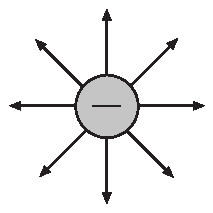
\includegraphics[keepaspectratio]{June2001-Q25-B}}
        \wrongchoice{\includegraphics[keepaspectratio]{June2001-Q25-C}}
      \correctchoice{\includegraphics[keepaspectratio]{June2001-Q25-D}}
    \end{choices}
    \end{multicols}
\end{question}
}

\element{nysed}{
\begin{question}{June2001-Q27}
    Which graph best represents the relationship between potential difference across a metallic conductor and the resulting current through the conductor at a constant temperature?
    \begin{multicols}{2}
    \begin{choices}
        \AMCboxDimensions{down=-2.5em}
        \correctchoice{
            \begin{tikzpicture}
                \begin{axis}[
                    axis y line=left,
                    axis x line=bottom,
                    axis line style={->},
                    xlabel={current},
                    xtick=\empty,
                    ylabel={potential},
                    ytick=\empty,
                    xmin=0,xmax=11,
                    ymin=0,ymax=11,
                    width=\columnwidth,
                    very thin,
                ]
                \addplot[line width=1pt,domain=0:10]{x};
                \end{axis}
            \end{tikzpicture}
        }
        \wrongchoice{
            \begin{tikzpicture}
                \begin{axis}[
                    axis y line=left,
                    axis x line=bottom,
                    axis line style={->},
                    xlabel={current},
                    xtick=\empty,
                    ylabel={potential},
                    ytick=\empty,
                    xmin=0,xmax=11,
                    ymin=0,ymax=11,
                    width=\columnwidth,
                    very thin,
                ]
                \addplot[line width=1pt,domain=0:10]{0.1*x*x};
                \end{axis}
            \end{tikzpicture}
        }
        \wrongchoice{
            \begin{tikzpicture}
                \begin{axis}[
                    axis y line=left,
                    axis x line=bottom,
                    axis line style={->},
                    xlabel={current},
                    xtick=\empty,
                    ylabel={potential},
                    ytick=\empty,
                    xmin=0,xmax=11,
                    ymin=0,ymax=11,
                    width=\columnwidth,
                    very thin,
                ]
                \addplot[line width=1pt,domain=0:10]{8};
                \end{axis}
            \end{tikzpicture}
        }
        \wrongchoice{
            \begin{tikzpicture}
                \begin{axis}[
                    axis y line=left,
                    axis x line=bottom,
                    axis line style={->},
                    xlabel={current},
                    xtick=\empty,
                    ylabel={potential},
                    ytick=\empty,
                    xmin=0,xmax=11,
                    ymin=0,ymax=11,
                    width=\columnwidth,
                    very thin,
                ]
                \addplot[line width=1pt,domain=0:10]{10/x};
                \end{axis}
            \end{tikzpicture}
        }
    \end{choices}
    \end{multicols}
\end{question}
}



%% Section Jan2001
%%--------------------
\element{nysed}{
\begin{question}{Jan2001-Q21}
    Metal sphere $A$ has a charge of \num[retain-explicit-plus]{+12} elementary charges and identical sphere $B$ has a charge of \num[retain-explicit-plus]{+16} elementary charges.
    After the two spheres are brought into contact, the charge on sphere $A$ is:
    \begin{choices}
        \wrongchoice{\num{-2} elementary charges}
        \wrongchoice{\num[retain-explicit-plus]{+2} elementary charges}
      \correctchoice{\num[retain-explicit-plus]{+14} elementary charges}
        \wrongchoice{\num[retain-explicit-plus]{+28} elementary charges}
    \end{choices}
\end{question}
}

\element{nysed}{
\begin{question}{Jan2001-Q22}
    Electrostatic force $F$ exists between two point charges.
    If the distance between the charges is tripled,
        the force between the charges will be:
    \begin{multicols}{4}
    \begin{choices}
      \correctchoice{$\dfrac{F}{9}$}
        \wrongchoice{$\dfrac{F}{3}$}
        \wrongchoice{$3 F$}
        \wrongchoice{$9 F$}
    \end{choices}
    \end{multicols}
\end{question}
}

\element{nysed}{
\begin{question}{Jan2001-Q23}
    Which net charge could be found on an object?
    \begin{multicols}{2}
    \begin{choices}
      \correctchoice{\SI[retain-explicit-plus]{+3.2e-18}{\coulomb}}
        \wrongchoice{\SI[retain-explicit-plus]{+2.4e-19}{\coulomb}}
        \wrongchoice{\SI{-1.8e-18}{\coulomb}}
        \wrongchoice{\SI{-0.80e-19}{\coulomb}}
    \end{choices}
    \end{multicols}
\end{question}
}

\element{nysed}{
\begin{question}{Jan2001-Q24}
    In the diagram below, two identical spheres,
        $A$ and $B$, have equal net positive charges.
    \begin{center}
    \begin{tikzpicture}
        \foreach \x in {0,90,180,270} {
            \draw[thick] (-2,0) -- ++(\x:0.5ex);
            \draw[thick] (+2,0) -- ++(\x:0.5ex);
        }
        \draw (-2,0) circle (1ex);
        \draw (+2,0) circle (1ex);
        \node[anchor=south] at (-2,1ex) {$A$};
        \node[anchor=south] at (+2,1ex) {$B$};
        \fill (0,2) circle (2pt) node[anchor=north] {$P$};
    \end{tikzpicture}
    \end{center}
    Which arrow best represents the direction of their electric field at point $P$?
    \begin{multicols}{2}
    \begin{choices}
        \AMCboxDimensions{down=-0.8cm}
        \wrongchoice{
            \begin{tikzpicture}[scale=2]
                \draw[dashed,white!60!black] (0,0) rectangle (1,1);
                \draw[thick,->] (0,0.5) -- (1,0.5);
            \end{tikzpicture}
        }
        \wrongchoice{
            \begin{tikzpicture}[scale=2]
                \draw[dashed,white!60!black] (0,0) rectangle (1,1);
                \draw[thick,->] (0.85,0.15) -- (0.15,0.85);
            \end{tikzpicture}
        }
        \wrongchoice{
            \begin{tikzpicture}[scale=2]
                \draw[dashed,white!60!black] (0,0) rectangle (1,1);
                \draw[thick,->] (0.15,0.15) -- (0.85,0.85);
            \end{tikzpicture}
        }
        \correctchoice{
            \begin{tikzpicture}[scale=2]
                \draw[dashed,white!60!black] (0,0) rectangle (1,1);
                \draw[thick,->] (0.5,0) -- (0.5,1);
            \end{tikzpicture}
        }
    \end{choices}
    \end{multicols}
\end{question}
}

\element{nysed}{
\begin{question}{Jan2001-Q25}
    How much work is done in moving \SI{5.0}{\coulomb} of charge against a potential difference of \SI{12}{\volt}?
    \begin{multicols}{2}
    \begin{choices}
        \wrongchoice{\SI{2.4}{\joule}}
        \wrongchoice{\SI{12}{\joule}}
        \wrongchoice{\SI{30}{\joule}}
      \correctchoice{\SI{60}{\joule}}
    \end{choices}
    \end{multicols}
\end{question}
}

\element{nysed}{
\begin{question}{Jan2001-Q28}
    Identical charges $A$, $B$, and $C$ are located between two oppositely charged parallel plates,
        as shown in the diagram below.
    \begin{center}
    \begin{tikzpicture}
        %% Bottom
        \draw (0,0) rectangle (6,-1em);
        \foreach \x in {2,6,...,58} {
            \draw[thick] (\x mm,-0.5em) -- ++(0:0.5ex);
            \draw[thick] (\x mm,-0.5em) -- ++(180:0.5ex);
        }
        %% Top
        \draw (0,2) rectangle (6,2cm+1em);
        \foreach \x in {2,6,...,58} {
            \draw[thick] (\x mm,2cm+0.5em) -- ++(0:0.5ex);
            \draw[thick] (\x mm,2cm+0.5em) -- ++(180:0.5ex);
            \draw[thick] (\x mm,2cm+0.5em) -- ++(90:0.5ex);
            \draw[thick] (\x mm,2cm+0.5em) -- ++(270:0.5ex);
        }
        %% Identical Charges A, B and C
        \foreach \x/\y/\z in {1/1.33/A,3/1/B,5/0.66/C} {
            \draw[thick] (\x,\y) -- ++(0:0.5ex);
            \draw[thick] (\x,\y) -- ++(90:0.5ex);
            \draw[thick] (\x,\y) -- ++(180:0.5ex);
            \draw[thick] (\x,\y) -- ++(270:0.5ex);
            \draw (\x,\y) circle (1ex);
            \node[anchor=west,xshift=1ex] at (\x,\y) {$\z$};
        }
    \end{tikzpicture}
    \end{center}
    The magnitude of the force exerted on the charges by the electric field between the plates is:
    \begin{choices}
        \wrongchoice{least on $A$ and greatest on $C$}
        \wrongchoice{greatest on $A$ and least on $C$}
        \wrongchoice{the same on $A$ and  $B$, but less on $C$}
      \correctchoice{the same for $A$, $B$, and $C$}
    \end{choices}
\end{question}
}

\element{nysed}{
\begin{question}{Jan2001-Q31}
    A glass rod becomes positively charged when it is rubbed with silk.
    This net positive charge accumulates because the glass rod:
    \begin{multicols}{2}
    \begin{choices}
        \wrongchoice{gains electrons}
        \wrongchoice{gains protons}
      \correctchoice{loses electrons}
        \wrongchoice{loses protons}
    \end{choices}
    \end{multicols}
\end{question}
}


%% Section June2000
%%--------------------
\element{nysed}{
\begin{question}{June2000-Q22}
    Two aluminum spheres of identical mass and identical charge $q$ hang from strings of equal length.
    If the spheres are in equilibrium,
        which diagram best represents the direction of each force acting on the spheres?
    \begin{center}
    \begin{tabu}{X[l]}
        \toprule
        Key \\
        \midrule
        $F_s$ = Force (tension) in string \\
        $F_e$ = Electrostatic force \\
        $F_g$ = Gravitational force \\
        \bottomrule
    \end{tabu}
    \end{center}
    %% NOTE: TODO: look at this
    \begin{multicols}{2}
    \begin{choices}
        \AMCboxDimensions{down=-2.5em}
        %\wrongchoice{
        %    \begin{tikzpicture}
        %        %% NOTE: TODO: draw tikz
        %    \end{tikzpicture}
        %}
        \wrongchoice{\includegraphics[keepaspectratio,scale=0.60]{June2000-Q22-A}}
        \wrongchoice{\includegraphics[keepaspectratio,scale=0.60]{June2000-Q22-B}}
        \wrongchoice{\includegraphics[keepaspectratio,scale=0.60]{June2000-Q22-C}}
      \correctchoice{\includegraphics[keepaspectratio,scale=0.60]{June2000-Q22-D}}
    \end{choices}
    \end{multicols}
\end{question}
}

\element{nysed}{
\begin{question}{June2000-Q23}
    Moving \SI{2.0}{\coulomb} of charge a distance of \SI{6.0}{\meter} from point $A$ to point $B$ within an electric field requires a \SI{5.0}{\newton} force.
    What is the electric potential difference between points $A$ and $B$?
    \begin{multicols}{2}
    \begin{choices}
        \wrongchoice{\SI{60}{\volt}}
        \wrongchoice{\SI{30}{\volt}}
      \correctchoice{\SI{15}{\volt}}
        \wrongchoice{\SI{2.5}{\volt}}
    \end{choices}
    \end{multicols}
\end{question}
}

\element{nysed}{
\begin{question}{June2000-Q24}
    A metal sphere having an excess of \num[retain-explicit-plus]{+5} elementary charges has a net electric charge of:
    \begin{multicols}{2}
    \begin{choices}
        \wrongchoice{\SI{1.6e-19}{\coulomb}}
      \correctchoice{\SI{8.0e-19}{\coulomb}}
        \wrongchoice{\SI{5.0e0}{\coulomb}}
        \wrongchoice{\SI{3.2e19}{\coulomb}}
    \end{choices}
    \end{multicols}
\end{question}
}

%% NOTE: alternative: what is the charge on $Y$ or $X$?
\element{nysed}{
\begin{question}{June2000-Q28}
    The diagram below shows the initial charge and position of three metal spheres, $X$, $Y$, and $Z$, on insulating stands.
    \begin{center}
    \begin{tikzpicture}
        \begin{scope}[xshift=-2cm]
            \draw[shading=ball,ball color=white!98!black] (0,0) circle (0.5);
            \node[anchor=center] at (0,0) {$X$};
            \draw[fill=white!60!black] (-0.05,-0.5) rectangle (0.05,-1);
            \draw[fill=white!60!black] (-0.5,-1.2) parabola bend (0,-1) (0.5,-1.2);
            \node[anchor=south] at (0,0.5) {\SI{+4e-6}{\coulomb}};
        \end{scope}
        \begin{scope}
            \draw[shading=ball,ball color=white!98!black] (0,0) circle (0.5);
            \node[anchor=center] at (0,0) {$Y$};
            \draw[fill=white!60!black] (-0.05,-0.5) rectangle (0.05,-1);
            \draw[fill=white!60!black] (-0.5,-1.2) parabola bend (0,-1) (0.5,-1.2);
            \node[anchor=south] at (0,0.5) {\SI{0}{\coulomb}};
        \end{scope}
        \begin{scope}[xshift=+2cm]
            \draw[shading=ball,ball color=white!98!black] (0,0) circle (0.5);
            \node[anchor=center] at (0,0) {$Z$};
            \draw[fill=white!60!black] (-0.05,-0.5) rectangle (0.05,-1);
            \draw[fill=white!60!black] (-0.5,-1.2) parabola bend (0,-1) (0.5,-1.2);
            \node[anchor=south] at (0,0.5) {\SI{0}{\coulomb}};
        \end{scope}
    \end{tikzpicture}
    \end{center}
    Sphere $X$ is brought into contact with sphere $Y$ and then removed.
    Then sphere $Y$ is brought into contact with sphere $Z$ and removed.
    What is the charge on sphere $Z$ after this procedure is completed?
    \begin{multicols}{2}
    \begin{choices}
      \correctchoice{\SI[retain-explicit-plus]{+1e-6}{\coulomb}}
        \wrongchoice{\SI[retain-explicit-plus]{+2e-6}{\coulomb}}
        \wrongchoice{\SI[retain-explicit-plus]{+3e-6}{\coulomb}}
        \wrongchoice{\SI[retain-explicit-plus]{+4e-6}{\coulomb}}
    \end{choices}
    \end{multicols}
\end{question}
}


\element{nysed}{
\begin{question}{June2000-Q30}
    Gravitational field strength is to \si{\newton\per\kilo\gram} as electric field strength is to:
    \begin{multicols}{4}
    \begin{choices}
        \wrongchoice{\si{\coulomb\per\joule}}
        \wrongchoice{\si{\coulomb\per\newton}}
        \wrongchoice{\si{\joule\per\coulomb}}
      \correctchoice{\si{\newton\per\coulomb}}
    \end{choices}
    \end{multicols}
\end{question}
}

\element{nysed}{
\begin{question}{June2000-Q33}
    The graph below shows the relationship between the work done on a charged body in an electric field and the net charge on the body.
    \begin{center}
    \begin{tikzpicture}
        \begin{axis}[
            axis y line=left,
            axis x line=bottom,
            axis line style={->},
            xlabel={Charge},
            xtick=\empty,
            ylabel={Work},
            ytick=\empty,
            xmin=0,xmax=10,
            ymin=0,ymax=10,
            width=0.90\columnwidth,
            height=0.45\columnwidth,
            very thin,
        ]
        \addplot[line width=1pt,domain=0:10]{x};
        \end{axis}
    \end{tikzpicture}
    \end{center}
    What does the slope of this graph represent?
    \begin{choices}
        \wrongchoice{power}
      \correctchoice{potential difference}
        \wrongchoice{force}
        \wrongchoice{electric field intensity}
    \end{choices}
\end{question}
}


%% Section June1999
%%--------------------

%% NOTE: Q25 requires graphics

\element{nysed}{
\begin{question}{June1999-Q26}
    Compared to the charge on a proton,
        the charge on an electron has the:
    \begin{choices}
        \wrongchoice{opposite sign and a smaller magnitude}
      \correctchoice{opposite sign and the same magnitude}
        \wrongchoice{same sign and a smaller magnitude}
        \wrongchoice{same sign and the same magnitude}
    \end{choices}
\end{question}
}

\element{nysed}{
\begin{question}{June1999-Q27}
    A point charge of \SI[retain-explicit-plus]{+3.0e-7}{\coulomb} is placed \SI{2.0e-2}{\meter} from a second point charge of \SI[retain-explicit-plus]{+4.0e-7}{\coulomb}.
    The magnitude of the electrostatic force between the charges is:
    \begin{multicols}{2}
    \begin{choices}
      \correctchoice{\SI{2.7}{\newton}}
        \wrongchoice{\SI{5.4e-2}{\newton}}
        \wrongchoice{\SI{3.0e-10}{\newton}}
        \wrongchoice{\SI{6.0e-12}{\newton}}
    \end{choices}
    \end{multicols}
\end{question}
}

%% NOTE: June1999-Q28 required graphic, tikz?
%% NOTE: June1999-Q29 required graphic

\element{nysed}{
\begin{question}{June1999-Q30}
    If \SI{15}{\joule} of work is required to move \SI{3.0}{\coulomb} of charge between two points,
        the potential difference between these two points is:
    \begin{multicols}{2}
    \begin{choices}
        \wrongchoice{\SI{45}{\volt}}
        \wrongchoice{\SI{15}{\volt}}
        \wrongchoice{\SI{3.0}{\volt}}
      \correctchoice{\SI{5.0}{\volt}}
    \end{choices}
    \end{multicols}
\end{question}
}

\element{nysed}{
\begin{question}{June1999-Q78}
    What did Millikan conclude after performing his oil-drop experiment?
    \begin{choices}
        \wrongchoice{The charge on an electron is \SI{1.0}{\coulomb}}
        \wrongchoice{The mass of an electron is \SI{1.7e-27}{\kilo\gram}}
      \correctchoice{The charge of any oil drop is an integer multiple of the charge on an electron}
        \wrongchoice{The charge on an oil drop may have any value larger than \SI{1.6e-19}{\coulomb}}
    \end{choices}
\end{question}
}


%% Section June1998
%%--------------------
\element{nysed}{
\begin{question}{June1998-Q22}
    Two plastic rods, $A$ and $B$, each posses a net negative charge of \SI{1.0e-3}{\coulomb}.
    The rods and a positively charged sphere are positioned as shown below.
    \begin{center}
    %% NOTE: TODO: fix charges on rod A
    \begin{tikzpicture}
        %% rod A
        \begin{scope}[xshift=-1cm]
            \draw (-2,0.5) -- (-0.5,0.5) -- (0,0) -- (-0.5,-0.5) -- (-2,-0.5);
            \node[anchor=center] at (-2,0) {$A$};
            \foreach \x in {-0.33,-0.66,-1.00,-1.33}
                \foreach \y in {-0.33,0,0.33}
                    \draw[thick] (\x,\y) -- ++(0:1ex);
        \end{scope}
        %% rod B
        \begin{scope}[yshift=-1cm]
            \draw (-0.5,-2) -- (-0.5,-0.5) -- (0,0) -- (0.5,-0.5) -- (0.5,-2);
            \node[anchor=center] at (0,-2) {$B$};
            \foreach \y in {-0.50,-0.75,-1.0,-1.25}
                \foreach \x in {-0.3,+0.20}
                    \draw[thick] (\x,\y) -- ++(0:1ex);
        \end{scope}
        %% sphere +
        \foreach \x in {0,90,180,270}
            \draw[thick] (0,0) -- ++(\x:1ex);
        \draw[thick] (0,0) circle (1em);
    \end{tikzpicture}
    \end{center}
    Which vector best represents the resultant electrostatic force on the sphere?
    \begin{multicols}{2}
    \begin{choices}
        \AMCboxDimensions{down=-0.8cm}
        \correctchoice{
            \begin{tikzpicture}[scale=2]
                \draw[dashed,white!60!black] (0,0) rectangle (1,1);
                \draw[thick,->] (0.15,0.15) -- (0.85,0.85);
            \end{tikzpicture}
        }
        \wrongchoice{
            \begin{tikzpicture}[scale=2]
                \draw[dashed,white!60!black] (0,0) rectangle (1,1);
                \draw[thick,->] (0.5,1) -- (0.5,0);
            \end{tikzpicture}
        }
        \wrongchoice{
            \begin{tikzpicture}[scale=2]
                \draw[dashed,white!60!black] (0,0) rectangle (1,1);
                \draw[thick,->] (0.5,0) -- (0.5,1);
            \end{tikzpicture}
        }
        \wrongchoice{
            \begin{tikzpicture}[scale=2]
                \draw[dashed,white!60!black] (0,0) rectangle (1,1);
                \draw[thick,->] (0.85,0.15) -- (0.15,0.85);
            \end{tikzpicture}
        }
    \end{choices}
    \end{multicols}
\end{question}
}

\element{nysed}{
\begin{question}{June1998-Q23}
    A sphere has a net excess charge of \SI{-4.8e-19}{\coulomb}.
    The sphere must have an excess of:
    \begin{multicols}{2}
    \begin{choices}
        \wrongchoice{1 electron}
        \wrongchoice{1 proton}
      \correctchoice{3 electrons}
        \wrongchoice{3 protons}
    \end{choices}
    \end{multicols}
\end{question}
}

\element{nysed}{
\begin{question}{June1998-Q24}
    The diagram below shows two metal spheres suspended by strings and separated by a distance of \SI{3.0}{\meter}.
    The charge on sphere $A$ is \SI[retain-explicit-plus]{+5.0e-4}{\coulomb} and the charge on sphere $B$ is \SI[retain-explicit-plus]{+3.0e-5}{\coulomb}.
    \begin{center}
    \begin{tikzpicture}
        %% ceiling
        \draw (-3,0) -- (3,0);
        \node[anchor=south,pattern=north east lines,minimum width=6cm] at (0,0) {};
        %% sphere A
        \node[thick,draw,circle,anchor=center] (A) at (-2,-3) {$A$};
        \draw[thick] (-2,0) -- (A.north);
        %% sphere B
        \node[thick,draw,circle,anchor=center] (B) at (+2,-3) {$B$};
        \draw[thick] (+2,0) -- (B.north);
        %% distance
        \draw[<->,shorten <=1pt,shorten >=1pt] (-2,-1) -- (2,-1) node[pos=0.5,anchor=center,fill=white] {\SI{3.0}{\meter}};
    \end{tikzpicture}
    \end{center}
    Which statement best describes the electrical force between the spheres?
    \begin{choices}
      \correctchoice{It has a magnitude of \SI{15}{\newton} and is repulsive.}
        \wrongchoice{It has a magnitude of \SI{45}{\newton} and is repulsive.}
        \wrongchoice{It has a magnitude of \SI{15}{\newton} and is attractive.}
        \wrongchoice{It has a magnitude of \SI{45}{\newton} and is attractive.}
    \end{choices}
\end{question}
}

\element{nysed}{
\begin{question}{June1998-Q25}
    Which diagram best represents the electic field near a positively charged conducting sphere?
    \begin{multicols}{2}
    \begin{choices}
        \AMCboxDimensions{down=-0.8cm}
        \wrongchoice{
            \begin{tikzpicture}[scale=1.33]
                \draw[dashed,white!60!black] (-1,-1) rectangle (1,1);
                \draw (0,0) circle (0.25);
                \foreach \x in {0,90,180,270} \draw[thick] (0,0) -- ++(\x:0.5ex);
                \foreach \y in {0,45,...,315} \draw[thick,latex-] (\y:0.25) -- ++(\y:0.75);
            \end{tikzpicture}
        }
        \correctchoice{
            \begin{tikzpicture}[scale=1.33]
                \draw[dashed,white!60!black] (-1,-1) rectangle (1,1);
                \draw (0,0) circle (0.25);
                \foreach \x in {0,90,180,270} \draw[thick] (0,0) -- ++(\x:0.5ex);
                \foreach \y in {0,45,...,315} \draw[thick,-latex] (\y:0.25) -- ++(\y:0.75);
            \end{tikzpicture}
        }
        \wrongchoice{
            \begin{tikzpicture}[scale=1.33]
                \draw[dashed,white!60!black] (-1,-1) rectangle (1,1);
                \draw (0,0) circle (0.25);
                \foreach \x in {0,90,180,270}\draw[thick] (0,0) -- ++(\x:0.5ex);
                \foreach \x in {0.60,0.90} {
                    \draw[thick,-latex] (-\x,0) arc(180:0:\x);
                    \draw[thick,-latex] (+\x,0) arc(360:180:\x);
                }
            \end{tikzpicture}
        }
        \wrongchoice{
            \begin{tikzpicture}[scale=1.33]
            \begin{scope}[decoration={markings,mark=at position 0.5 with {\arrow{latex}}}]
                \draw[dashed,white!60!black] (-1,-1) rectangle (1,1);
                \clip (-1,-1) rectangle (1,1);
                \draw (0,0) circle (0.25);
                \foreach \x in {0,90,180,270} \draw[thick] (0,0) -- ++(\x:0.5ex);
                %% +/- 30
                \draw[thick,postaction={decorate}] (120:0.25) .. controls ++(120:1) and ++(240:1) .. (240:0.25);
                \draw[thick,postaction={decorate}] (60:0.25) .. controls ++(60:1) and ++(300:1) .. (300:0.25);
                %% +/- 10
                \draw[thick,postaction={decorate}] (100:0.25) .. controls ++(120:2) and ++(240:2) .. (260:0.25);
                \draw[thick,postaction={decorate}] (80:0.25) .. controls ++(60:2) and ++(300:2) .. (280:0.25);
            \end{scope}
            \end{tikzpicture}
        }
    \end{choices}
    \end{multicols}
\end{question}
}

\element{nysed}{
\begin{question}{June1998-Q26}
    Two oppositely charges parallel plates are a fixed distance apart.
    Which graph best represents the relationship between the electric field intensity between the plates and the potential difference across the plates?
    \begin{multicols}{2}
    \begin{choices}
        \AMCboxDimensions{down=-2.5em}
        \correctchoice{
            \begin{tikzpicture}
                \begin{axis}[
                    axis y line=left,
                    axis x line=bottom,
                    axis line style={->},
                    xlabel={electric field},
                    xtick=\empty,
                    ylabel={potential},
                    ytick=\empty,
                    xmin=0,xmax=11,
                    ymin=0,ymax=11,
                    width=\columnwidth,
                    very thin,
                ]
                \addplot[line width=1pt,domain=0:10]{x};
                \end{axis}
            \end{tikzpicture}
        }
        \wrongchoice{
            \begin{tikzpicture}
                \begin{axis}[
                    axis y line=left,
                    axis x line=bottom,
                    axis line style={->},
                    xlabel={electric field},
                    xtick=\empty,
                    ylabel={potential},
                    ytick=\empty,
                    xmin=0,xmax=11,
                    ymin=0,ymax=11,
                    width=\columnwidth,
                    very thin,
                ]
                \addplot[line width=1pt,domain=0:10]{10/x};
                \end{axis}
            \end{tikzpicture}
        }
        \wrongchoice{
            \begin{tikzpicture}
                \begin{axis}[
                    axis y line=left,
                    axis x line=bottom,
                    axis line style={->},
                    xlabel={electric field},
                    xtick=\empty,
                    ylabel={potential},
                    ytick=\empty,
                    xmin=0,xmax=11,
                    ymin=0,ymax=11,
                    width=\columnwidth,
                    very thin,
                ]
                \addplot[line width=1pt,domain=0:10]{8};
                \end{axis}
            \end{tikzpicture}
        }
        \wrongchoice{
            \begin{tikzpicture}
                \begin{axis}[
                    axis y line=left,
                    axis x line=bottom,
                    axis line style={->},
                    xlabel={electric field},
                    xtick=\empty,
                    ylabel={potential},
                    ytick=\empty,
                    xmin=0,xmax=11,
                    ymin=0,ymax=11,
                    width=\columnwidth,
                    very thin,
                ]
                \addplot[line width=1pt,domain=0:10]{0.1*x*x};
                \end{axis}
            \end{tikzpicture}
        }
    \end{choices}
    \end{multicols}
\end{question}
}


%% Section June1997
%%--------------------
\element{nysed}{
\begin{question}{June1997-Q22}
    When a plastic rod is rubbed with wool,
        the wool acquires a positive charge because:
    \begin{choices}
      \correctchoice{electrons are transferred from the wool to the rod.}
        \wrongchoice{protons are transferred from the wool to the rod.}
        \wrongchoice{electrons are transferred from the rod to the wool.}
        \wrongchoice{protons are transferred from the rod to the wool.}
    \end{choices}
\end{question}
}

\element{nysed}{
\begin{question}{June1997-Q23}
    Three identical metal spheres are mounted on insulating stands.
    Initially, sphere $A$ has a net charge of $q$ and spheres $B$ and $C$ are uncharged.
    Sphere $A$ is touched to sphere $B$ and removed.
    Then sphere $A$ is touched to sphere $C$ and removed.
    What is the final charge on sphere $A$?
    \begin{multicols}{4}
    \begin{choices}
        \wrongchoice{$q$}
        \wrongchoice{$\dfrac{q}{2}$}
        \wrongchoice{$\dfrac{q}{3}$}
      \correctchoice{$\dfrac{q}{4}$}
    \end{choices}
    \end{multicols}
\end{question}
}

\element{nysed}{
\begin{question}{June1997-Q24}
    A distance of \SI{1.0e3}{\meter} separates the charge at the bottom of a cloud and the ground.
    The electric field intensity between the bottom of the cloud and the ground is \SI{2.0e4}{\newton\per\coulomb}.
    What is the potential difference between the bottom of the cloud and the ground?
    \begin{multicols}{2}
    \begin{choices}
        \wrongchoice{\SI{1.3e23}{\volt}}
        \wrongchoice{\SI{2.0e1}{\volt}}
      \correctchoice{\SI{2.0e7}{\volt}}
        \wrongchoice{\SI{5.0e-2}{\volt}}
    \end{choices}
    \end{multicols}
\end{question}
}

%% NOTE: June1997-Q25 tikz

\element{nysed}{
\begin{question}{June1997-Q26}
    What is the net static electric charge on a metal sphere having an excess of \num[retain-explicit-plus]{+3} elementary charges?
    \begin{multicols}{2}
    \begin{choices}
        \wrongchoice{\SI{1.6e-19}{\coulomb}}
      \correctchoice{\SI{4.8e-19}{\coulomb}}
        \wrongchoice{\SI{3.0e0}{\coulomb}}
        \wrongchoice{\SI{4.8e19}{\coulomb}}
    \end{choices}
    \end{multicols}
\end{question}
}

\element{nysed}{
\begin{question}{June1997-Q30}
    Which is a vector quantity?
    \begin{choices}
        \wrongchoice{electric charge}
        \wrongchoice{electric resistance}
        \wrongchoice{electric potential difference}
      \correctchoice{electric field intensity}
    \end{choices}
\end{question}
}


%% Section June1996
%%--------------------
\element{nysed}{
\begin{question}{June1996-Q23}
    A repulsive electrostatic force of magnitude $F$ exists between two metal spheres having identical charge $q$.
    The distance between their centers is $r$.
    Which combination of changes would produce \emph{no} change in the electrostatic force between the spheres?
    \begin{choices}
        \wrongchoice{doubling $q$ on one sphere while doubling $r$}
      \correctchoice{doubling $q$ on both spheres while doubling $r$}
        \wrongchoice{doubling $q$ on one sphere while halving $r$}
        \wrongchoice{doubling $q$ on both spheres while halving $r$}
    \end{choices}
\end{question}
}

\element{nysed}{
\begin{question}{June1996-Q24}
    An inflated balloon which has been rubbed against a person's hair is touched to a neutral wall and remains attracted to it.
    Which diagram best represents the charge distribution on the balloon and wall?
    \begin{multicols}{2}
    \begin{choices}
        %% NOTE: TODO: finish drawing Balloon and charges
        \AMCboxDimensions{down=-1cm}
        \wrongchoice{
            \begin{tikzpicture}
                %% balloon
                \draw (-1ex,0) to[out=90,in=270] (-1,2) arc (180:0:1) to[out=270,in=90] (+1ex,0);
                \draw[thick] (0,0) circle (1.0ex and 0.25ex);
                \node[anchor=center] at (0,2) {Balloon};
                %% wall
                \draw[thick] (2,0) -- (1,0) -- (1,3) -- (2,3);
                \node[anchor=north west] at (1,3) {Wall};
            \end{tikzpicture}
        }
    \end{choices}
    \end{multicols}
\end{question}
}

\element{nysed}{
\begin{question}{June1996-Q25}
    Two metal spheres having charges of \SI[retain-explicit-plus]{+4.0e-6}{\coulomb} and \SI[retain-explicit-plus]{+2.0e-5}{\coulomb},
        respectively, are brought into contact and then separated.
    After separation, the charge on each sphere is:
    \begin{multicols}{2}
    \begin{choices}
        \wrongchoice{\SI{8.0e-11}{\coulomb}}
        \wrongchoice{\SI{8.0e-6}{\coulomb}}
        \wrongchoice{\SI{2.1e-6}{\coulomb}}
      \correctchoice{\SI{1.2e-5}{\coulomb}}
    \end{choices}
    \end{multicols}
\end{question}
}


\element{nysed}{
\begin{question}{June1996-Q26}
    Which graph best represents the relationship between the magnitude of the electric field strength around a point charge and the distance from the point charge?
    %% NOTE: dup of June2004-Q45
    \begin{multicols}{2}
    \begin{choices}
        \AMCboxDimensions{down=-2.5em}
        \wrongchoice{
            \begin{tikzpicture}
                \begin{axis}[
                    axis y line=left,
                    axis x line=bottom,
                    axis line style={->},
                    xlabel={distance},
                    xtick=\empty,
                    ylabel={electric field},
                    ytick=\empty,
                    xmin=0,xmax=11,
                    ymin=0,ymax=11,
                    width=\columnwidth,
                    very thin,
                ]
                \addplot[line width=1pt,domain=0:10]{8};
                \end{axis}
            \end{tikzpicture}
        }
        \wrongchoice{
            \begin{tikzpicture}
                \begin{axis}[
                    axis y line=left,
                    axis x line=bottom,
                    axis line style={->},
                    xlabel={distance},
                    xtick=\empty,
                    ylabel={electric field},
                    ytick=\empty,
                    xmin=0,xmax=11,
                    ymin=0,ymax=11,
                    width=\columnwidth,
                    very thin,
                ]
                \addplot[line width=1pt,domain=0:10]{x};
                \end{axis}
            \end{tikzpicture}
        }
        \correctchoice{
            \begin{tikzpicture}
                \begin{axis}[
                    axis y line=left,
                    axis x line=bottom,
                    axis line style={->},
                    xlabel={distance},
                    xtick=\empty,
                    ylabel={electric field},
                    ytick=\empty,
                    xmin=0,xmax=11,
                    ymin=0,ymax=11,
                    width=\columnwidth,
                    very thin,
                ]
                \addplot[line width=1pt,domain=0:10]{10/x/x};
                \end{axis}
            \end{tikzpicture}
        }
        \wrongchoice{
            \begin{tikzpicture}
                \begin{axis}[
                    axis y line=left,
                    axis x line=bottom,
                    axis line style={->},
                    xlabel={distance},
                    xtick=\empty,
                    ylabel={electric field},
                    ytick=\empty,
                    xmin=0,xmax=11,
                    ymin=0,ymax=11,
                    width=\columnwidth,
                    very thin,
                ]
                \addplot[line width=1pt,domain=0:10]{0.1*x*x};
                \end{axis}
            \end{tikzpicture}
        }
    \end{choices}
    \end{multicols}
\end{question}
}

\element{nysed}{
\begin{question}{June1996-Q27}
    Moving \SI[retain-explicit-plus]{+2.0}{\coulomb} of charge from infinity to point $P$ in an electric field requires \SI{8.0}{\joule} of work.
    What is the electric potential at point $P$?
    \begin{multicols}{2}
    \begin{choices}
        \wrongchoice{\SI{0.25}{\volt}}
      \correctchoice{\SI{8.0}{\volt}}
        \wrongchoice{\SI{16}{\volt}}
        \wrongchoice{\SI{4.0}{\volt}}
    \end{choices}
    \end{multicols}
\end{question}
}

\element{nysed}{
\begin{question}{June1996-Q28}
    What is the magnitude of the electrostatic force experienced by one elementary charge at a point in an electric field where the electric field intensity is \SI{3.0e3}{\newton\per\coulomb}?
    \begin{multicols}{2}
    \begin{choices}
        \wrongchoice{\SI{1.0e3}{\newton}}
        \wrongchoice{\SI{1.6e-19}{\newton}}
        \wrongchoice{\SI{3.0e3}{\newton}}
      \correctchoice{\SI{4.8e-16}{\newton}}
    \end{choices}
    \end{multicols}
\end{question}
}


%% Section June1995
%%--------------------
\element{nysed}{
\begin{question}{June1995-Q21}
    The diagram below shows the arrangement of three charged hollow metal spheres, $A$, $B$, and $C$.
    The arrows indicate the direction of the electric forces acting between the spheres.
    At least two of the sphere are positively charged.
    \begin{center}
    \begin{tikzpicture}
        %% NOTE: duplicate graphic from Jan2002-Q25
        %% coordinates
        \coordinate (A) at (0,3);
        \coordinate (B) at (-1.73,0);
        \coordinate (C) at (+1.73,0);
        %% sphere A
        \node[draw,circle,anchor=center] at (A) {$A$};
        \draw[very thick,->] (A.center) ++(240:1em) -- ++(240:1);
        \draw[very thick,->] (A.center) ++(300:1em) -- ++(300:1);
        %% sphere B
        \node[draw,circle,anchor=center] at (B) {$B$};
        \draw[very thick,->] (B.center) ++(60:1em) -- ++(60:1);
        \draw[very thick,->] (B.center) ++(180:1em) -- ++(180:1);
        %% sphere C
        \node[draw,circle,anchor=center] at (C) {$C$};
        \draw[very thick,->] (C.center) ++(0:1em) -- ++(0:1);
        \draw[very thick,->] (C.center) ++(120:1em) -- ++(120:1);
    \end{tikzpicture}
    \end{center}
    Which sphere, if any, could be negatively charged?
    \begin{multicols}{2}
    \begin{choices}
      \correctchoice{sphere $A$}
        \wrongchoice{sphere $B$}
        \wrongchoice{sphere $C$}
        \wrongchoice{no sphere}
    \end{choices}
    \end{multicols}
\end{question}
}

\element{nysed}{
\begin{question}{June1995-Q22}
    The diagram below shows the initial charge and position of three identical metal spheres, $X$, $Y$, and $Z$,
        which have been placed on insulating stands.
    \begin{center}\small
    \begin{tikzpicture}
        \begin{scope}[xshift=-3cm]
            \draw[shading=ball,ball color=white!98!black] (0,0) circle (0.5);
            \node[anchor=center] at (0,0) {$X$};
            \draw[fill=white!60!black] (-0.05,-0.5) rectangle (0.05,-1);
            \draw[fill=white!60!black] (-0.5,-1.2) parabola bend (0,-1) (0.5,-1.2);
            \node[anchor=south] at (0,0.5) {\SI{+2e-6}{\coulomb}};
        \end{scope}
        \begin{scope}
            \draw[shading=ball,ball color=white!98!black] (0,0) circle (0.5);
            \node[anchor=center] at (0,0) {$Y$};
            \draw[fill=white!60!black] (-0.05,-0.5) rectangle (0.05,-1);
            \draw[fill=white!60!black] (-0.5,-1.2) parabola bend (0,-1) (0.5,-1.2);
            \node[anchor=south] at (0,0.5) {\SI{+4e-6}{\coulomb}};
        \end{scope}
        \begin{scope}[xshift=+3cm]
            \draw[shading=ball,ball color=white!98!black] (0,0) circle (0.5);
            \node[anchor=center] at (0,0) {$Z$};
            \draw[fill=white!60!black] (-0.05,-0.5) rectangle (0.05,-1);
            \draw[fill=white!60!black] (-0.5,-1.2) parabola bend (0,-1) (0.5,-1.2);
            \node[anchor=south] at (0,0.5) {\SI{+6e-6}{\coulomb}};
        \end{scope}
    \end{tikzpicture}
    \end{center}
    All three spheres are simultaneously brought into contact with each other and then returned to their original positions.
    Which statement best describes the charge of the spheres after this procedure is completed?
    \begin{choices}
        \wrongchoice{All the spheres are neutral}
      \correctchoice{Each sphere has a net charge of \SI{4e-6}{\coulomb}}
        \wrongchoice{Each sphere retains the same charge they had originally}
        \wrongchoice{Sphere $Y$ has a greater charge than sphere $X$ or $Y$.}
    \end{choices}
\end{question}
}

\element{nysed}{
\begin{question}{June1995-Q23}
    Which diagram best represents the electric field of a point charge?
    \begin{multicols}{2}
    \begin{choices}
        \AMCboxDimensions{down=-1.2cm}
        %% ANS is 1
        \correctchoice{
            \begin{tikzpicture}
                \draw[dashed,white!60!black] (-1.5,-1.5) rectangle (1.5,1.5);
                %% positive charge
                \foreach \x in {0,90,180,270}
                    \draw (0,0) -- ++(\x:0.1cm);
                \draw (0,0) circle (0.15cm);
                %% field lines
                \foreach \x in {0,45,90,...,315} {
                    \draw[thick,-latex] (0,0) ++(\x:0.15cm) -- (\x:1cm);
                    \draw[thick] (\x:1cm) -- (\x:1.5cm);
                }
            \end{tikzpicture}
        }
        \wrongchoice{
            \begin{tikzpicture}
                \draw[dashed,white!60!black] (-1.5,-1.5) rectangle (1.5,1.5);
                %% positive charge
                \foreach \x in {0,90,180,270}
                    \draw (0,0) -- ++(\x:0.1cm);
                \draw (0,0) circle (0.15cm);
                %% field lines
                \foreach \x in {0,45,90,...,315} {
                    \draw[thick] (0,0) ++(\x:0.15cm) -- (\x:0.75cm);
                    \draw[thick,-latex] (\x:1.5cm) -- (\x:0.75cm);
                }
            \end{tikzpicture}
        }
        \wrongchoice{
            \begin{tikzpicture}
                \draw[dashed,white!60!black] (-1.5,-1.5) rectangle (1.5,1.5);
                %% positive charge
                \foreach \x in {0,90,180,270}
                    \draw (0,0) -- ++(\x:0.1cm);
                \draw (0,0) circle (0.15cm);
                %% field lines
                \foreach \x in {0.66,1.33} {
                    \draw[thick,-latex] (0,\x) arc(90:270:\x);
                    \draw[thick,-latex] (0,-\x) arc(270:450:\x);
                }
            \end{tikzpicture}
        }
        \wrongchoice{
            \begin{tikzpicture}
                \draw[dashed,white!60!black] (-1.5,-1.5) rectangle (1.5,1.5);
                %% positive charge
                \foreach \x in {0,90,180,270}
                    \draw (0,0) -- ++(\x:0.1cm);
                \draw (0,0) circle (0.15cm);
                %% field lines
                \foreach \x in {0.66,1.33} {
                    \draw[thick,latex-] (0,\x) arc(90:270:\x);
                    \draw[thick,latex-] (0,-\x) arc(270:450:\x);
                }
            \end{tikzpicture}
        }
    \end{choices}
    \end{multicols}
\end{question}
}

\element{nysed}{
\begin{question}{June1995-Q24}
    If \SI{20}{\joule} of work is done in transferring \SI{5.0}{\coulomb} of charge between two points,
        the potential difference between these two points is:
    \begin{multicols}{2}
    \begin{choices}
        \wrongchoice{\SI{100}{\volt}}
        \wrongchoice{\SI{50}{\volt}}
        \wrongchoice{\SI{0.25}{\volt}}
      \correctchoice{\SI{4.0}{\volt}}
    \end{choices}
    \end{multicols}
\end{question}
}


%% Section June1994
%%--------------------
\element{nysed}{
\begin{question}{June1994-Q23}
    As shown in the diagram below,
        a neutral pith ball suspended on a string is attracted to a positively charged rod.
    \begin{center}
    \begin{tikzpicture}
        %% ceiling
        \draw (-2,0) -- (2,0);
        \node[anchor=south,minimum width=4cm,pattern=north east lines] at (0,0) {};
        %% Pith Ball
        \draw (0,0) -- (240:3);
        \draw[fill=white!60!black] (240:3) circle (1ex) node[anchor=west,xshift=1ex] {Pith Ball};
        %% Rod
        \begin{scope}[shift={(240:4)}]
            \draw (-0.3,-1) rectangle (0.3,2);
            \node[anchor=east] at (-0.3,-1) {Rod};
            \foreach \x in {-8,-4,...,16}
                \foreach \y in {0,90,180,270}
                    \draw[thick] (0,\x mm) -- ++(\y:0.1);
        \end{scope}
    \end{tikzpicture}
    \end{center}
    During contact with the rod, the pith ball:
    \begin{multicols}{2}
    \begin{choices}
      \correctchoice{loses electrons}
        \wrongchoice{gains electrons}
        \wrongchoice{loses protons}
        \wrongchoice{gains protons}
    \end{choices}
    \end{multicols}
\end{question}
}

\element{nysed}{
\begin{question}{June1994-Q24}
    The electrostatic force between two positive point charges is $F$ when the charges are 0.1 meter apart.
    When these point charges are placed 0.05 meter apart,
        the electrostatic force between then is:
    \begin{multicols}{2}
    \begin{choices}
        \wrongchoice{$4F$, and attracting}
        \wrongchoice{$\dfrac{F}{4}$, and attracting}
      \correctchoice{$4F$, and repelling}
        \wrongchoice{$\dfrac{F}{4}$, and repelling}
    \end{choices}
    \end{multicols}
\end{question}
}

\element{nysed}{
\begin{question}{June1994-Q25}
    An electron is located \SI{1.0}{\meter} from a \SI{+2.0}{\coulomb} charge,
        as shown in the diagram below.
    \begin{center}
    \begin{tikzpicture}
        %% 2.0 C charge
        \node[draw,circle,anchor=center] (A) at (-2,0) {\small \SI{+2.0}{\coulomb}};
        %% electron
        \node[draw,circle,anchor=center] (B) at (+2,0) {\footnotesize $e^-$};
        %% distance
        \draw[dashed] (A.south) -- (-2,-1.25);
        \draw[dashed] (B.south) -- (+2,-1.25);
        \draw[thick,<->] (-2,-1) -- (2,-1) node[pos=0.5,anchor=center,fill=white] {\SI{1.0}{\meter}};
        %% options
        \foreach \x/\y in {90/A,0/B,180/D,270/C}
            \fill (2,0) ++ (\x:2) circle (1.5pt) node[anchor=south] {$\y$};
    \end{tikzpicture}
    \end{center}
    The electrostatic force acting on the electron is directed toward point:
    \begin{multicols}{4}
    \begin{choices}[o]
        \wrongchoice{$A$}
        \wrongchoice{$B$}
        \wrongchoice{$C$}
      \correctchoice{$D$}
    \end{choices}
    \end{multicols}
\end{question}
}

\element{nysed}{
\begin{question}{June1994-Q26}
    What is the magnitude of the electric force acting on an electron located in an electric field with an intensity of \SI{5.0e3}{\newton\per\coulomb}?
    \begin{multicols}{2}
    \begin{choices}
        \wrongchoice{\SI{3.2e-23}{\newton}}
      \correctchoice{\SI{8.0e-16}{\newton}}
        \wrongchoice{\SI{5.0e3}{\newton}}
        \wrongchoice{\SI{3.2e22}{\newton}}
    \end{choices}
    \end{multicols}
\end{question}
}

\element{nysed}{
\begin{question}{June1994-Q27}
    The unit ``volt per meter (\si{\volt\per\meter})'' measures the same quantity as:
    \begin{choices}
        \wrongchoice{joule per volt (\si{\joule\per\volt})}
        \wrongchoice{newton per ampere-meter (\si{\newton\per\ampere\per\meter})}
        \wrongchoice{newton meter squared per coulomb squared (\si{\newton\meter\squared\per\coulomb\squared})}
      \correctchoice{newton per coulomb (\si{\newton\per\coulomb})}
    \end{choices}
\end{question}
}


%% Section June1990
%%--------------------
\element{nysed}{
\begin{question}{June1990-Q24}
    Sphere $A$ has a charge of \SI{+2e-6}{\coulomb} and is brought into contact with a similar sphere, $B$,
        which has a charge of \SI{-4e-6}{\coulomb}.
    After it is separated from sphere $B$,
        sphere $A$ will have a charge of:
    \begin{multicols}{2}
    \begin{choices}
      \correctchoice{\SI{-1e-6}{\coulomb}}
        \wrongchoice{\SI{-2e-6}{\coulomb}}
        \wrongchoice{\SI{+2e-6}{\coulomb}}
        \wrongchoice{\SI{+6e-6}{\coulomb}}
    \end{choices}
    \end{multicols}
\end{question}
}

\element{nysed}{
\begin{question}{June1990-Q26}
    An alpha particle with a charge of $+2$ elementary charges is accelerated by a potential difference of \SI{1.0e6}{\volt}.
    The energy acquired by the particle is:
    \begin{multicols}{2}
    \begin{choices}
        \wrongchoice{\SI{0.50e6}{\eV}}
      \correctchoice{\SI{2.0e6}{\eV}}
        \wrongchoice{\SI{1.60e-19}{\eV}}
        \wrongchoice{\SI{3.2e-13}{\eV}}
    \end{choices}
    \end{multicols}
\end{question}
}

\element{nysed}{
\begin{question}{June1990-Q28}
    If the charge on each of the two small spheres a fixed distance apart is doubled,
        the force of attraction between the spheres will be:
    \begin{multicols}{2}
    \begin{choices}
        \wrongchoice{quartered}
        \wrongchoice{doubled}
        \wrongchoice{halved}
      \correctchoice{quadrupled}
    \end{choices}
    \end{multicols}
\end{question}
}

\element{nysed}{
\begin{question}{June1990-Q29}
    What is the magnitude of the electric field intensity at a point in the field where an electron experiences a \SI{1.0}{\newton} force?
    \begin{multicols}{2}
    \begin{choices}
        \wrongchoice{\SI{1.0}{\newton\per\coulomb}}
        \wrongchoice{\SI{1.6e-19}{\newton\per\coulomb}}
      \correctchoice{\SI{6.3e18}{\newton\per\coulomb}}
        \wrongchoice{\SI{9.1e-31}{\newton\per\coulomb}}
    \end{choices}
    \end{multicols}
\end{question}
}


%% Section June1989
%%--------------------
\element{nysed}{
\begin{question}{June1989-Q27}
    A negatively charged object is brought near the knob of a negatively charged electroscope.
    The leaves of the electroscope will:
    \begin{choices}
        \wrongchoice{move closer together}
      \correctchoice{move farther apart}
        \wrongchoice{become positively charged}
        \wrongchoice{become neutral}
    \end{choices}
\end{question}
}

\element{nysed}{
\begin{question}{June1989-Q28}
    Sphere $A$ carries a charge of \SI{+2}{\coulomb} and an identical sphere $B$ is neutral.
    If the spheres touch one another and then are separated,
        the charge on sphere $B$ would be:
    \begin{multicols}{2}
    \begin{choices}
      \correctchoice{\SI{+1}{\coulomb}}
        \wrongchoice{\SI{+2}{\coulomb}}
        \wrongchoice{\SI{0}{\coulomb}}
        \wrongchoice{\SI{+4}{\coulomb}}
    \end{choices}
    \end{multicols}
\end{question}
}

\element{nysed}{
\begin{question}{June1989-Q29}
    Which procedure will double the force between two point charges?
    \begin{choices}
        \wrongchoice{doubling the distance between the charges}
      \correctchoice{doubling the magnitude of one charge}
        \wrongchoice{halving the distance between the charges}
        \wrongchoice{halving the magnitude of one charge}
    \end{choices}
\end{question}
}

\element{nysed}{
\begin{question}{June1989-Q30}
    How much energy is required to move \SI{3.2e-19}{\coulomb} of charge through a potential difference of \SI{5}{\volt}?
    \begin{multicols}{2}
    \begin{choices}
        \wrongchoice{\SI{5}{\eV}}
        \wrongchoice{\SI{2}{\eV}}
      \correctchoice{\SI{10}{\eV}}
        \wrongchoice{\SI{20}{\eV}}
    \end{choices}
    \end{multicols}
\end{question}
}

\element{nysed}{
\begin{question}{June1989-Q33}
    A glass rod is given a positive charge by rubbing it with silk.
    The rod has become positive by:
    \begin{multicols}{2}
    \begin{choices}
        \wrongchoice{gaining electrons}
        \wrongchoice{gaining protons}
      \correctchoice{losing electrons}
        \wrongchoice{losing protons}
    \end{choices}
    \end{multicols}
\end{question}
}


%% Section June1986
%%--------------------
\element{nysed}{
\begin{question}{June1986-Q32}
    The diagrams below represent cross sections of negatively charged rods.
    Which diagram best illustrates the electric field around the negatively charged rod?
    \begin{multicols}{2}
    \begin{choices}
        \AMCboxDimensions{down=-2.5em}
        \wrongchoice{
            \begin{tikzpicture}
                \draw[dashed,white!60!black] (-1.5,-1.5) rectangle (1.5,1.5);
                %% charge
                \draw (0,0) circle (1ex);
                \draw[thick] (-0.5ex,0) -- (0.5ex,0);
                %% field
                \foreach \x in {0,60,120}
                    \draw[thick,-latex] (\x:1.25ex) -- (\x:1.5);
                \foreach \x in {180,240,300}
                    \draw[thick,-latex] (\x:1.5) -- (\x:1.25ex);
            \end{tikzpicture}
        }
        \wrongchoice{
            \begin{tikzpicture}
                \draw[dashed,white!60!black] (-1.5,-1.5) rectangle (1.5,1.5);
                %% charge
                \draw (0,0) circle (1ex);
                \draw[thick] (-0.5ex,0) -- (0.5ex,0);
                %% field
                \foreach \x in {0,45,...,315}
                    \draw[thick,-latex] (\x:1.5ex) -- (\x:1.5);
            \end{tikzpicture}
        }
        %% ANS is 3
        \correctchoice{
            \begin{tikzpicture}
                \draw[dashed,white!60!black] (-1.5,-1.5) rectangle (1.5,1.5);
                %% charge
                \draw (0,0) circle (1ex);
                \draw[thick] (-0.5ex,0) -- (0.5ex,0);
                %% field
                \foreach \x in {0,45,...,315}
                    \draw[thick,-latex] (\x:1.5) -- (\x:1.25ex);
            \end{tikzpicture}
        }
        \wrongchoice{
            \begin{tikzpicture}
                \draw[dashed,white!60!black] (-1.5,-1.5) rectangle (1.5,1.5);
                %% charge
                \draw (0,0) circle (1ex);
                \draw[thick] (-0.5ex,0) -- (0.5ex,0);
                %% field
                \foreach \x in {0,120,240}
                    \draw[thick,-latex] (\x:1.25ex) -- (\x:1.5);
                \foreach \x in {60,180,300}
                    \draw[thick,-latex] (\x:1.5) -- (\x:1.25ex);
            \end{tikzpicture}
        }
    \end{choices}
    \end{multicols}
\end{question}
}

\element{nysed}{
\begin{question}{June1986-Q33}
    A neutral rubber rod is rubbed with fur and acquires a charge of \SI{-2e-6}{\coulomb}.
    The charge on the fur is:
    \begin{multicols}{2}
    \begin{choices}
        \wrongchoice{\SI{+1e-6}{\coulomb}}
      \correctchoice{\SI{+2e-6}{\coulomb}}
        \wrongchoice{\SI{-1e-6}{\coulomb}}
        \wrongchoice{\SI{-2e-6}{\coulomb}}
    \end{choices}
    \end{multicols}
\end{question}
}

\element{nysed}{
\begin{question}{June1986-Q34}
    A small, uncharged metal sphere is placed near a larger, negatively charges sphere.
    Which idagram best represents the charge distribution on the \emph{smaller} sphere?
    \begin{multicols}{2}
    \begin{choices}
        \AMCboxDimensions{down=-2.5em}
        \wrongchoice{
            \begin{tikzpicture}
                \draw[dashed,white!60!black] (-1.5,-1.5) rectangle (1.5,1.5);
                \begin{scope}[xshift=-0.75cm]
                    \draw (0,0) circle (0.66cm);
                    \draw[thick] (-0.25,0) -- (0.25,0);
                \end{scope}
                \begin{scope}[xshift=+0.75cm,scale=0.66]
                    \draw (0,0) circle (0.66cm);
                    \foreach \x in {-4,0,4} {
                        \foreach \z in {0,180}
                            \draw[thick] (-2mm, \x mm) -- ++(\z:0.5ex);
                        \foreach \z in {0,90,180,270}
                            \draw[thick] (2mm, \x mm) -- ++(\z:0.5ex);
                    }
                \end{scope}
            \end{tikzpicture}
        }
        \wrongchoice{
            \begin{tikzpicture}
                \draw[dashed,white!60!black] (-1.5,-1.5) rectangle (1.5,1.5);
                \begin{scope}[xshift=-0.75cm]
                    \draw (0,0) circle (0.66cm);
                    \draw[thick] (-0.25,0) -- (0.25,0);
                \end{scope}
                \begin{scope}[xshift=+0.75cm,scale=0.66]
                    \draw (0,0) circle (0.66cm);
                    \foreach \x/\y in {0/3,-2/-1,2/-1} {
                        \foreach \z in {0,90,180,270}
                            \draw[thick] (-\x mm, \y mm) -- ++(\z:0.5ex);
                    }
                    \foreach \x/\y in {-2/1,2/1,0/-3} {
                        \foreach \z in {0,180}
                            \draw[thick] (-\x mm, \y mm) -- ++(\z:0.5ex);
                    }
                \end{scope}
            \end{tikzpicture}
        }
        %% ANS is 3
        \correctchoice{
            \begin{tikzpicture}
                \draw[dashed,white!60!black] (-1.5,-1.5) rectangle (1.5,1.5);
                \begin{scope}[xshift=-0.75cm]
                    \draw (0,0) circle (0.66cm);
                    \draw[thick] (-0.25,0) -- (0.25,0);
                \end{scope}
                \begin{scope}[xshift=+0.75cm,scale=0.66]
                    \draw (0,0) circle (0.66cm);
                    \foreach \x in {-4,0,4} {
                        \foreach \z in {0,180}
                            \draw[thick] (2mm, \x mm) -- ++(\z:0.5ex);
                        \foreach \z in {0,90,180,270}
                            \draw[thick] (-2mm, \x mm) -- ++(\z:0.5ex);
                    }
                \end{scope}
            \end{tikzpicture}
        }
        \wrongchoice{
            \begin{tikzpicture}
                \draw[dashed,white!60!black] (-1.5,-1.5) rectangle (1.5,1.5);
                \begin{scope}[xshift=-0.75cm]
                    \draw (0,0) circle (0.66cm);
                    \draw[thick] (-0.25,0) -- (0.25,0);
                \end{scope}
                \begin{scope}[xshift=+0.75cm,scale=0.66]
                    \draw (0,0) circle (0.66cm);
                    \foreach \x/\y in {0/3,-2/-1,2/-1,-2/1,2/1,0/-3} {
                        \foreach \z in {0,180}
                            \draw[thick] (-\x mm, \y mm) -- ++(\z:0.5ex);
                    }
                \end{scope}
            \end{tikzpicture}
        }
    \end{choices}
    \end{multicols}
\end{question}
}

\element{nysed}{
\begin{question}{June1986-Q35}
    The electrical force of attraction between two point charges if $F$.
    The charge on one of the objects is \emph{quadrupled} and the charge on the other object is \emph{doubled}.
    The new force between the objects is:
    \begin{multicols}{4}
    \begin{choices}
        \wrongchoice{$6F$}
        \wrongchoice{$2F$}
        \wrongchoice{$\dfrac{F}{2}$}
      \correctchoice{$8F$}
    \end{choices}
    \end{multicols}
\end{question}
}

\element{nysed}{
\begin{question}{June1986-Q37}
    It takes \SI{15}{\joule} of work to bring \SI{3.0}{\coulomb} of positive charge from infinity to a point.
    What is the electric potential at this point in an electric field?
    \begin{multicols}{2}
    \begin{choices}
        \wrongchoice{\SI{45}{\volt}}
      \correctchoice{\SI{5.0}{\volt}}
        \wrongchoice{\SI{0.20}{\volt}}
        \wrongchoice{\SI{0}{\volt}}
    \end{choices}
    \end{multicols}
\end{question}
}

\element{nysed}{
\begin{question}{June1986-Q58}
    The diagram below represents a particle of mass $m$ and charge $+q$ located between two charged parallel plates.
    The electric field intensity between the plates is $E$.
    \begin{center}
    \begin{tikzpicture}
        %% particle
        \fill (3,1.5) circle (3pt) node[xshift=3pt,anchor=west] {$+q$};
        %% Bottom positive
        \draw (0,0) rectangle (6,-1em);
        \foreach \x in {2,6,...,58}
            \foreach \y in {0,90,180,270} {
                \draw[thick] (\x mm,-0.5em) -- ++(\y:0.5ex);
            }
        %% Top negative
        \draw (0,3) rectangle (6,3cm+1em);
        \foreach \x in {2,6,...,58}
            \foreach \y in {0,180} {
                \draw[thick] (\x mm,3cm+0.5em) -- ++(\y:0.5ex);
            }
    \end{tikzpicture}
    \end{center}
    The particle will remain stationary when:
    \begin{choices}
        \wrongchoice{$Eq$ is less than $mg$}
        \wrongchoice{$Eq$ is greater than $mg$}
      \correctchoice{$Eq$ equals $mg$}
    \end{choices}
\end{question}
}


\newcommand{\nysedJuneNineteenEightySixQNinetyOne}{
\begin{tikzpicture}
    %% Charge
    \fill (0,0) circle (2pt) node[anchor=center,shift={(202.5:1.5em)}] {$Q$};
    %% field lines
    \foreach \x in {0,45,...,315}
        \draw[thick,-latex] (0,0) -- (\x:2);
    %% point A and B
    \fill (67.5:1) circle (2pt) node[anchor=south west] {$A$};
    \fill (67.5:2) circle (2pt) node[anchor=south west] {$B$};
\end{tikzpicture}
}

\element{nysed}{
\begin{question}{June1986-Q91}
    The diagram below represents an object with a charge of \SI{+3}{\coulomb} located at point $Q$.
    The object produces an electric field as shown in the diagram.
    A small, positive test charge is located at point $A$.
    \begin{center}
        \nysedJuneNineteenEightySixQNinetyOne
    \end{center}
    The electric field intensity at point $A$, \SI{3.0}{\meter} from charge $Q$, is:
    \begin{multicols}{2}
    \begin{choices}
        \wrongchoice{\SI{1.0e9}{\newton\per\coulomb}}
        \wrongchoice{\SI{2.0e9}{\newton\per\coulomb}}
      \correctchoice{\SI{3.0e9}{\newton\per\coulomb}}
        \wrongchoice{\SI{9.0e9}{\newton\per\coulomb}}
    \end{choices}
    \end{multicols}
\end{question}
}

\element{nysed}{
\begin{question}{June1986-Q92}
    The diagram below represents an object with a charge of \SI{+3}{\coulomb} located at point $Q$.
    The object produces an electric field as shown in the diagram.
    A small, positive test charge is located at point $A$.
    \begin{center}
        \nysedJuneNineteenEightySixQNinetyOne
    \end{center}
    A small, positive test charge is moved from point $A$ to point $B$.
    Compared with the potential energy of the test charge at point $A$,
        the potential energy of the test charge at point $B$ is:
    \begin{multicols}{3}
    \begin{choices}
      \correctchoice{less}
        \wrongchoice{greater}
        \wrongchoice{the same}
    \end{choices}
    \end{multicols}
\end{question}
}

\element{nysed}{
\begin{question}{June1986-Q93}
    An electron is accelerated from rest through a potential difference of \SI{200}{\volt}.
    The work done on the electron is:
    \begin{multicols}{2}
    \begin{choices}
        \wrongchoice{\SI{8.00e-3}{\eV}}
        \wrongchoice{\SI{3.20e-17}{\eV}}
        \wrongchoice{\SI{320}{\eV}}
      \correctchoice{\SI{200}{\eV}}
    \end{choices}
    \end{multicols}
\end{question}
}


%% Section June1985
%%--------------------
\element{nysed}{
\begin{question}{June1985-Q33}
    Two identical conducting spheres carry charges of \SI{+3}{\coulomb} and \SI{-1}{\coulomb}, respectively.
    If the spheres are brought into contact and separated,
        the final charges on each will be:
    \begin{multicols}{2}
    \begin{choices}
      \correctchoice{\SI{+1}{\coulomb}}
        \wrongchoice{\SI{+2}{\coulomb}}
        \wrongchoice{\SI{-1}{\coulomb}}
        \wrongchoice{\SI{-2}{\coulomb}}
    \end{choices}
    \end{multicols}
\end{question}
}

\element{nysed}{
\begin{question}{June1985-Q34}
    An alpha particle with a charge of $+2$ elementary charges is accelerated in a vacuum through a potential difference of \SI{10 000}{\volt}.
    What is the energy acquired by the particle?
    \begin{multicols}{2}
    \begin{choices}
        \wrongchoice{\SI{3.2e-15}{\eV}}
        \wrongchoice{\SI{2.0}{\eV}}
      \correctchoice{\SI{20 000}{\eV}}
        \wrongchoice{\SI{40 000}{\eV}}
    \end{choices}
    \end{multicols}
\end{question}
}

\element{nysed}{
\begin{question}{June1985-Q36}
    Which diagram best illustrates a neutral electroscope being charge by conduction?
    \begin{multicols}{2}
    \begin{choices}[o]
        \AMCboxDimensions{down=-1.2cm}
        \wrongchoice{
            \begin{tikzpicture}
                \draw[dashed,white!60!black] (-1.5,-2) rectangle (1.5,1);
                \begin{scope}[xshift=-0.25cm]
                    \draw[thick] (-1.1,0.25) -- (0,0.25) -- (0,-0.25) -- (-1.1,-0.25);
                    \foreach \x in {0.25,0.75}
                        \foreach \z in {0,90,180,270}
                            \draw[thick] (-\x,0) -- ++(\z:0.66ex);
                \end{scope}
                \begin{scope}[xshift=0.5cm]
                    \draw[thick] (0,0) circle (0.50cm);
                    \draw[thick] (0,-0.5) -- (0,-1.25);
                    \draw[thick] (0,-1.25) -- ++(315:0.75);
                    \draw[thick] (0,-1.25) -- ++(225:0.75);
                    \foreach \x in {-0.75,0.75}
                        \foreach \z in {0,90,180,270}
                            \draw[thick] (-\x,-1.5) -- ++(\z:0.66ex);
                \end{scope}
            \end{tikzpicture}
        }
        \wrongchoice{
            \ctikzset{bipoles/length=0.75cm}
            \begin{tikzpicture}
                \draw[dashed,white!60!black] (-1.5,-2) rectangle (1.5,1);
                \begin{scope}[xshift=-0.25cm]
                    \draw[thick] (-1.1,0.25) -- (0,0.25) -- (0,-0.25) -- (-1.1,-0.25);
                    \foreach \x in {0.25,0.75}
                        \foreach \z in {0,180}
                            \draw[thick] (-\x,0) -- ++(\z:0.66ex);
                \end{scope}
                \begin{scope}[xshift=0.5cm]
                    \draw[thick] (0,0) circle (0.50cm);
                    \draw (0.5,0) -- (0.75,0) -- ++(270:0.5) node[ground] {};
                    \draw[thick] (0,-0.5) -- (0,-1.25);
                    \draw[thick] (0,-1.25) -- ++(315:0.75);
                    \draw[thick] (0,-1.25) -- ++(225:0.75);
                    \foreach \x in {-0.75,0.75}
                        \foreach \z in {0,90,180,270}
                            \draw[thick] (-\x,-1.5) -- ++(\z:0.66ex);
                \end{scope}
            \end{tikzpicture}
        }
        \wrongchoice{
            \begin{tikzpicture}
                \draw[dashed,white!60!black] (-1.5,-2) rectangle (1.5,1);
                \begin{scope}[xshift=-0.25cm]
                    \draw[thick] (-1.1,0.25) -- (0,0.25) -- (0,-0.25) -- (-1.1,-0.25);
                    \foreach \x in {0.25,0.75}
                        \foreach \z in {0,180}
                            \draw[thick] (-\x,0) -- ++(\z:0.66ex);
                \end{scope}
                \begin{scope}[xshift=0.25cm]
                    \draw[thick] (0,0) circle (0.50cm);
                    \draw[thick] (0,-0.5) -- (0,-1.25);
                    \draw[thick] (0,-1.25) -- ++(315:0.75);
                    \draw[thick] (0,-1.25) -- ++(225:0.75);
                    \foreach \x in {-0.75,0.75}
                        \foreach \z in {0,90,180,270}
                            \draw[thick] (-\x,-1.5) -- ++(\z:0.66ex);
                \end{scope}
            \end{tikzpicture}
        }
        %% ANS is 4
        \correctchoice{
            \begin{tikzpicture}
                \draw[dashed,white!60!black] (-1.5,-2) rectangle (1.5,1);
                \begin{scope}[xshift=-0.25cm]
                    \draw[thick] (-1.1,0.25) -- (0,0.25) -- (0,-0.25) -- (-1.1,-0.25);
                    \foreach \x in {0.25,0.75}
                        \foreach \z in {0,180}
                            \draw[thick] (-\x,0) -- ++(\z:0.66ex);
                \end{scope}
                \begin{scope}[xshift=0.25cm]
                    \draw[thick] (0,0) circle (0.50cm);
                    \draw[thick] (0,-0.5) -- (0,-1.25);
                    \draw[thick] (0,-1.25) -- ++(315:0.75);
                    \draw[thick] (0,-1.25) -- ++(225:0.75);
                    \foreach \x in {-0.75,0.75}
                        \foreach \z in {0,90,180,270}
                            \draw[thick] (-\x,-1.5) -- ++(\z:0.66ex);
                \end{scope}
            \end{tikzpicture}
        }
    \end{choices}
    \end{multicols}
\end{question}
}

\element{nysed}{
\begin{question}{June1985-Q37}
    If the magnitude of the charge on each of two positively charged objects is halved,
        the electrostatic force between the objects will:
    \begin{choices}
        \wrongchoice{decrease to one-half}
      \correctchoice{decrease to one-quarter}
        \wrongchoice{decrease to one-sixteenth}
        \wrongchoice{remain the same}
    \end{choices}
\end{question}
}

\element{nysed}{
\begin{question}{June1985-Q38}
    The diagram below shows some of the lines of electrical force around a positive charge.
    \begin{center}
    \begin{tikzpicture}[scale=0.80]
        %% charge
        \draw (0,0) circle (1ex);
        \draw[thick] (-0.55ex,0) -- (+0.55ex,0);
        \draw[thick] (0,-0.55ex) -- (0,+0.55ex);
        %% field
        \foreach \x in {0,45,...,315}
            \draw[thick,-latex,shorten <=1pt] ({\x-10}:1ex) -- ({\x-10}:3);
        %% labels
        \fill (80:0.5) circle (2pt) node[anchor=south west] {$A$};
        \fill (305:1.5) circle (2pt) node[anchor=south west] {$B$};
        \fill (260:2.5) circle (2pt) node[anchor=north west] {$C$};
    \end{tikzpicture}
    \end{center}
    The strength of the electric field is:
    \begin{choices}[o]
      \correctchoice{greatest at point $A$}
        \wrongchoice{greatest at point $B$}
        \wrongchoice{greatest at point $C$}
        \wrongchoice{equal at points $A$, $B$, and $C$}
    \end{choices}
\end{question}
}

\newcommand{\nysedJuneNineteenEightyFiveQNinetyOne}{
\begin{tikzpicture}
    %% X and Y
    \node[draw,circle,anchor=center] (X) at (-3,0) {$X$};
    \node[draw,circle,anchor=center] (Y) at (+3,0) {$Y$};
    \node[anchor=north] at (X.south) {\SI{+1.0e-6}{\coulomb}};
    \node[anchor=north] at (Y.south) {\SI{+1.0e-6}{\coulomb}};
    %% 3.0 m
    \draw[dashed] (X.north) -- ++(90:1);
    \draw[dashed] (Y.north) -- ++(90:1);
    \draw[thick,<->] (-3,0.9) -- (3,0.9) node[pos=0.5,anchor=center,fill=white] {\SI{3.0}{\meter}};
    %% options
    \fill (0,0) ++ (180:1.5) circle (2pt) node[anchor=south] {$B$};
    \fill (0,0) circle (2pt) node[anchor=south] {$C$};
    \fill (0,0) ++ (0:1.5) circle (2pt) node[anchor=south] {$D$};
    \fill (0,0) ++ (270:1) circle (2pt) node[anchor=south] {$A$};
\end{tikzpicture}
}

\element{nysed}{
\begin{question}{June1985-Q91}
    The diagram below represents two charges spheres, $X$ and $Y$.
    \begin{center}
        \nysedJuneNineteenEightyFiveQNinetyOne
    \end{center}
    At which point is the magnitude of the electric field equal to zero?
    \begin{multicols}{4}
    \begin{choices}
        \wrongchoice{$A$}
        \wrongchoice{$B$}
      \correctchoice{$C$}
        \wrongchoice{$D$}
    \end{choices}
    \end{multicols}
\end{question}
}

\element{nysed}{
\begin{question}{June1985-Q92}
    The diagram below represents two charges spheres, $X$ and $Y$.
    \begin{center}
        \nysedJuneNineteenEightyFiveQNinetyOne
    \end{center}
    At which point is the magnitude of the electric field equal to zero?
    \begin{multicols}{2}
    \begin{choices}
        \AMCboxDimensions{down=-1.2cm}
        \wrongchoice{
            \begin{tikzpicture}[scale=2]
                \draw[dashed,white!60!black] (0,0) rectangle (1,1);
                \draw[thick,-latex] (0.85,0.85) -- (0.15,0.15);
            \end{tikzpicture}
        }
        \wrongchoice{
            \begin{tikzpicture}[scale=2]
                \draw[dashed,white!60!black] (0,0) rectangle (1,1);
                \draw[thick,-latex] (0.15,0.85) -- (0.85,0.15);
            \end{tikzpicture}
        }
        \wrongchoice{
            \begin{tikzpicture}[scale=2]
                \draw[dashed,white!60!black] (0,0) rectangle (1,1);
                \draw[thick,-latex] (0.5,0) -- (0.5,1);
            \end{tikzpicture}
        }
        %% ANS is 4
        \correctchoice{
            \begin{tikzpicture}[scale=2]
                \draw[dashed,white!60!black] (0,0) rectangle (1,1);
                \draw[thick,-latex] (0.5,1) -- (0.5,0);
            \end{tikzpicture}
        }
    \end{choices}
    \end{multicols}
\end{question}
}

\element{nysed}{
\begin{question}{June1985-Q93}
    The diagram below represents two charges spheres, $X$ and $Y$.
    \begin{center}
        \nysedJuneNineteenEightyFiveQNinetyOne
    \end{center}
    If a unit positive charge moves directly from point $B$ to point $D$,
        the potential energy of the charge will:
    \begin{choices}
        \wrongchoice{decrease, only}
        \wrongchoice{increase, only}
      \correctchoice{decrease then increase}
        \wrongchoice{increase then decrease}
    \end{choices}
\end{question}
}

\element{nysed}{
\begin{question}{June1985-Q94}
    The diagram below represents two charges spheres, $X$ and $Y$.
    \begin{center}
        \nysedJuneNineteenEightyFiveQNinetyOne
    \end{center}
    The magnitude of the force between the two spheres is:
    \begin{multicols}{2}
    \begin{choices}
      \correctchoice{\SI{1.0e-3}{\newton}}
        \wrongchoice{\SI{1.0e3}{\newton}}
        \wrongchoice{\SI{3.0e-3}{\newton}}
        \wrongchoice{\SI{3.0e3}{\newton}}
    \end{choices}
    \end{multicols}
\end{question}
}

\element{nysed}{
\begin{question}{June1985-Q95}
    The diagram below represents two charges spheres, $X$ and $Y$.
    \begin{center}
        \nysedJuneNineteenEightyFiveQNinetyOne
    \end{center}
    Moving the two spheres toward each other would cause their electrical potential energy to:
    \begin{choices}
        \wrongchoice{decrease}
      \correctchoice{increase}
        \wrongchoice{remain the same}
    \end{choices}
\end{question}
}

\element{nysed}{
\begin{question}{June1985-Q96}
    The diagram below represents two charges spheres, $X$ and $Y$.
    \begin{center}
        \nysedJuneNineteenEightyFiveQNinetyOne
    \end{center}
    Compared to the force of the electric field of sphere $X$ on sphere $Y$,
        the force of the electric field of sphere $Y$ on sphere $X$ is:
    \begin{multicols}{3}
    \begin{choices}
        \wrongchoice{less}
        \wrongchoice{greater}
      \correctchoice{the same}
    \end{choices}
    \end{multicols}
\end{question}
}


\endinput


